\documentclass[11pt]{article} 
\usepackage{geometry}
\usepackage{setspace}
\usepackage{newtxtext,newtxmath}
\usepackage{graphicx}
\usepackage{itshape}
\usepackage{float}
\usepackage{amsmath}
\usepackage{subcaption}

\geometry{
    letterpaper,
    margin=0.75in
}

\begin{document} 
\singlespacing

\section{Question 1}
Done. See code.

\section{Question 2}
Done. See code. 

The definition of admissible is that it's always less than or equal to the true cost. In other words, it must be optimistic. Because in the problem statement the cost for diagonal or grid-aligned movements are both 1.0, that means our heuristic can't just be the euclidean distance (since that would be an overestimation of the diagonal cost).

Instead we use the exact cost it would be if there were no obstacles between ourselves and the goal which can be computed in a closed-form manner. That is, moving diagonally until we are axis-aligned with the goal, and then moving straight toward the goal. Because this uses the actual movement cost, but with no obstacles, we guarantee that the heuristic will always be less than or equal to the real cost.

\begin{equation}
	h = min(abs(g.x - s.x), abs(g.y - s.y)) + abs(abs(g.x - s.x) - abs(g.y - s.y))
\end{equation}

The first term is the diagonal move, and the second term is the remainder of the distance to the goal as a straight-line move

\section{Question 3}

\begin{figure}[H]
	\centering
    	\begin{subfigure}{0.33\textwidth}
    		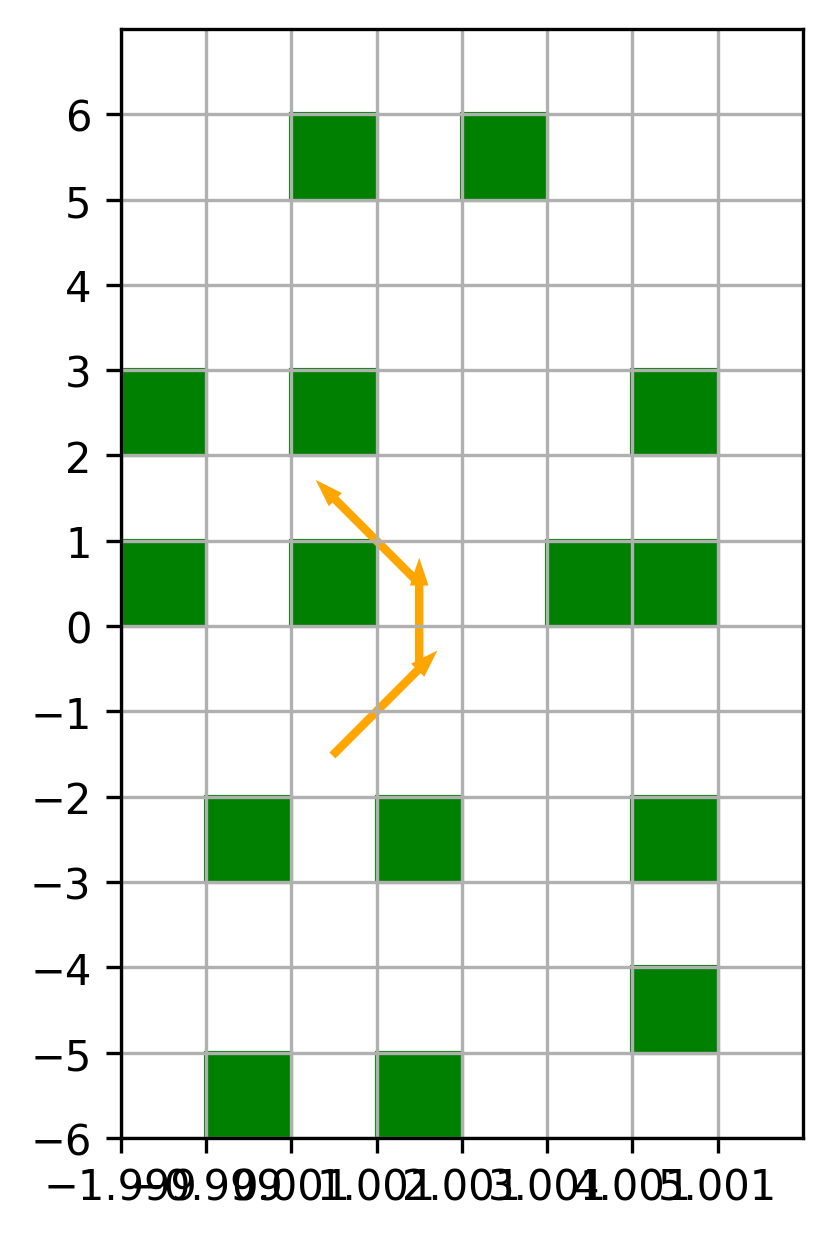
\includegraphics[width=1.0\textwidth]{"outputs/q3: #1.png"}
    		\caption{Q3  Plan A.}
	\end{subfigure}
    	\begin{subfigure}{0.33\textwidth}
    		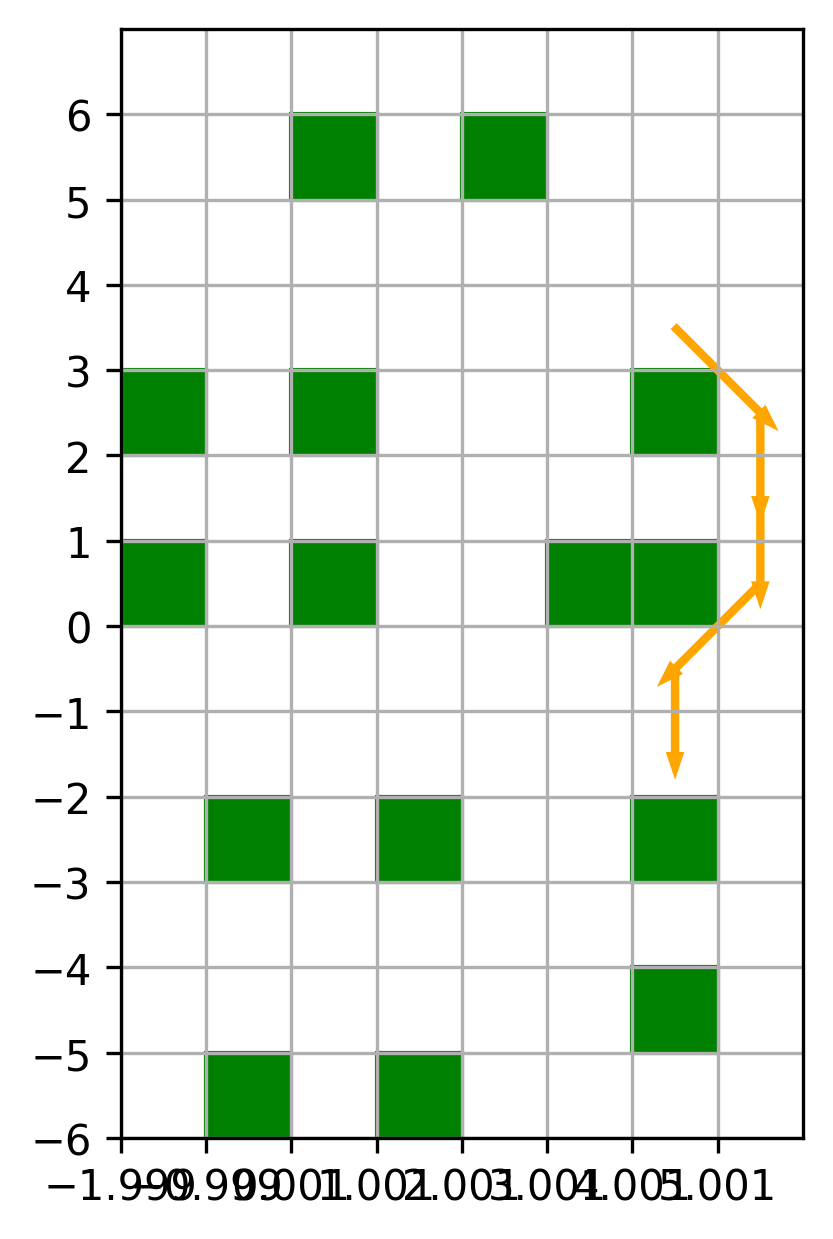
\includegraphics[width=1.0\textwidth]{"outputs/q3: #2.png"}
    		\caption{Q3  Plan B.}
	\end{subfigure}
    	\begin{subfigure}{0.33\textwidth}
    		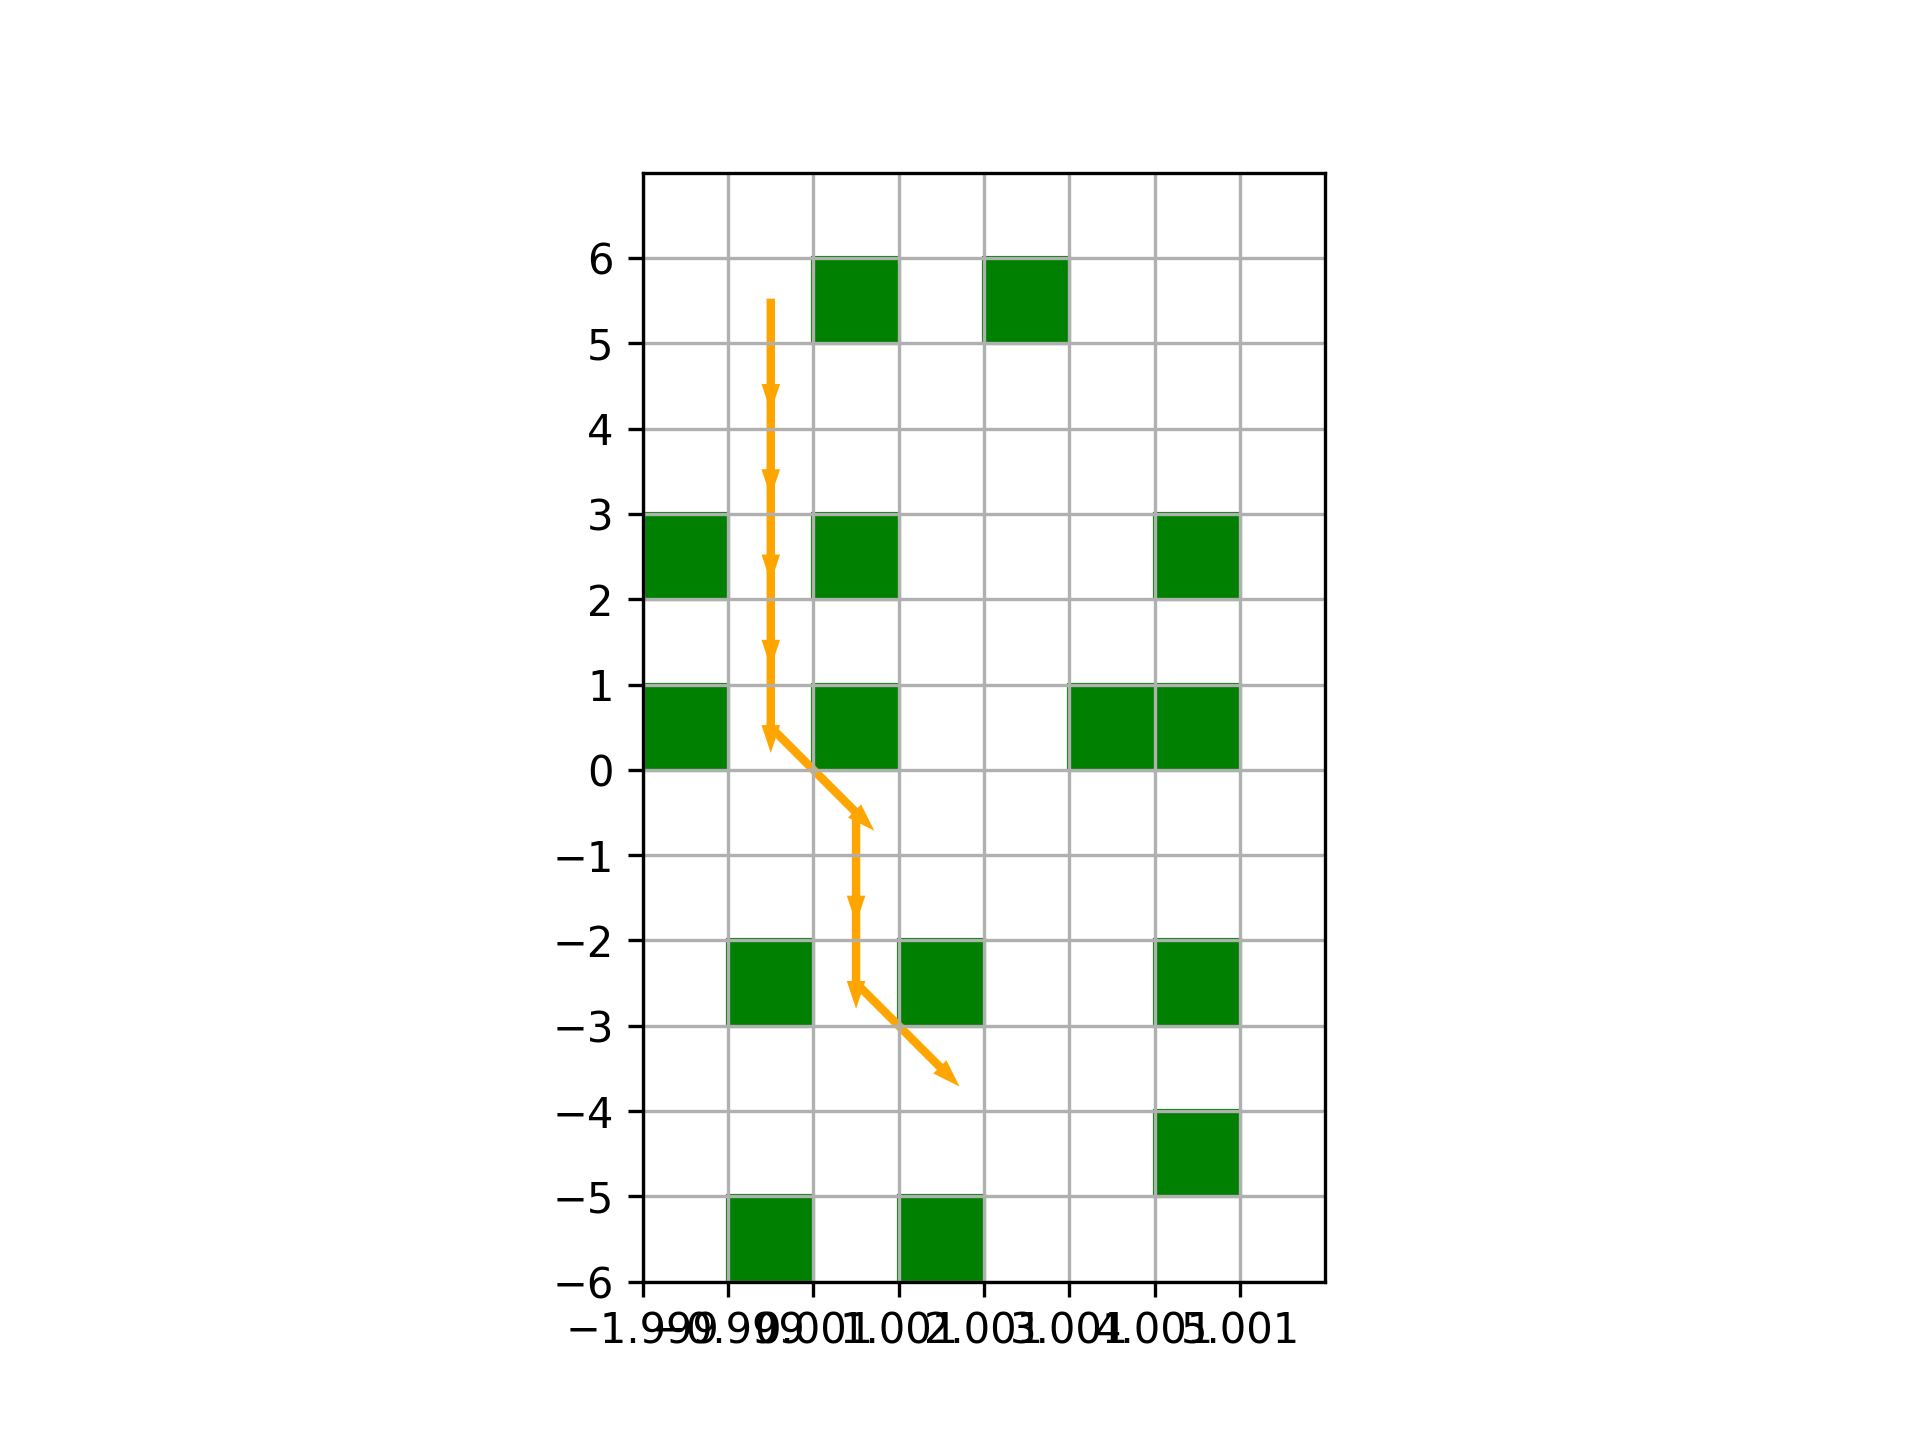
\includegraphics[width=1.0\textwidth]{"outputs/q3: #3.png"}
    		\caption{Q3  Plan C.}
	\end{subfigure}
	
\end{figure}


\section{Question 4}
Done. See code.

The way I solved this problem was by creating an online-planner class which takes a robot, a map, and a planner as input. I also added \textit{unexplored} variables to each \textit{Node} class. 

For this question I created a \textit{GridRobot} which moves instantaneously from cell to cell

The cost for a node is then 1.0 if it's either free or unexplored (we assume the unexplored map is free), or 1000.0 if it's occupied.

Lastly, the online planner will iteratively plan, move the robot, observe the neighbors, and then update the map before repeating. So no change had to be made to the set of expanded nodes (besides adding the aforementioned \textit{unexplored} variable)

When using an online A* with a sensing model, it means there's a chance our robot falls into a "trap", meaning that it could pursue a very promising direct route, only to find out there's walls in the way. The time it would take to sense the walls and plan around them would reduce the robot's time-to-goal compared to if it had complete environmental knowledge.


\section{Question 5}

\begin{figure}[H]
    \centering
    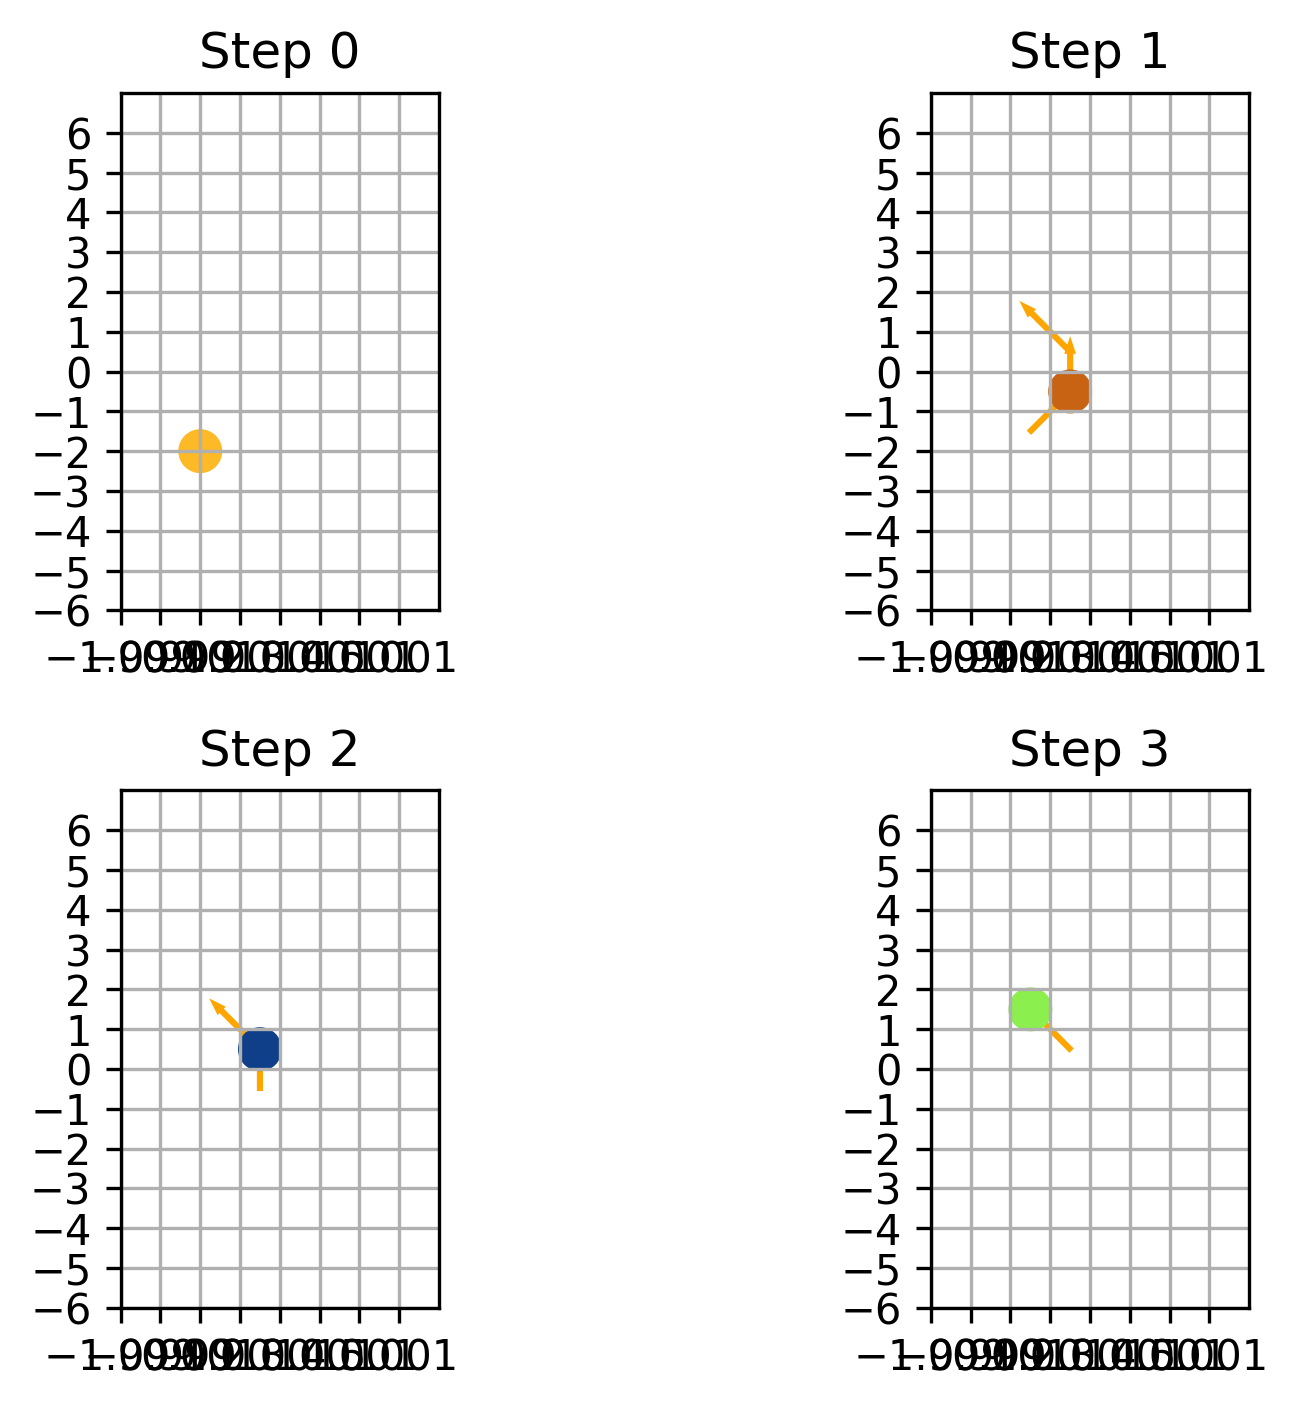
\includegraphics[width=0.4\textwidth]{"outputs/q5: #1.png"}
    \caption{Q5  Plan A.}
\end{figure}

\begin{figure}[H]
    \centering
    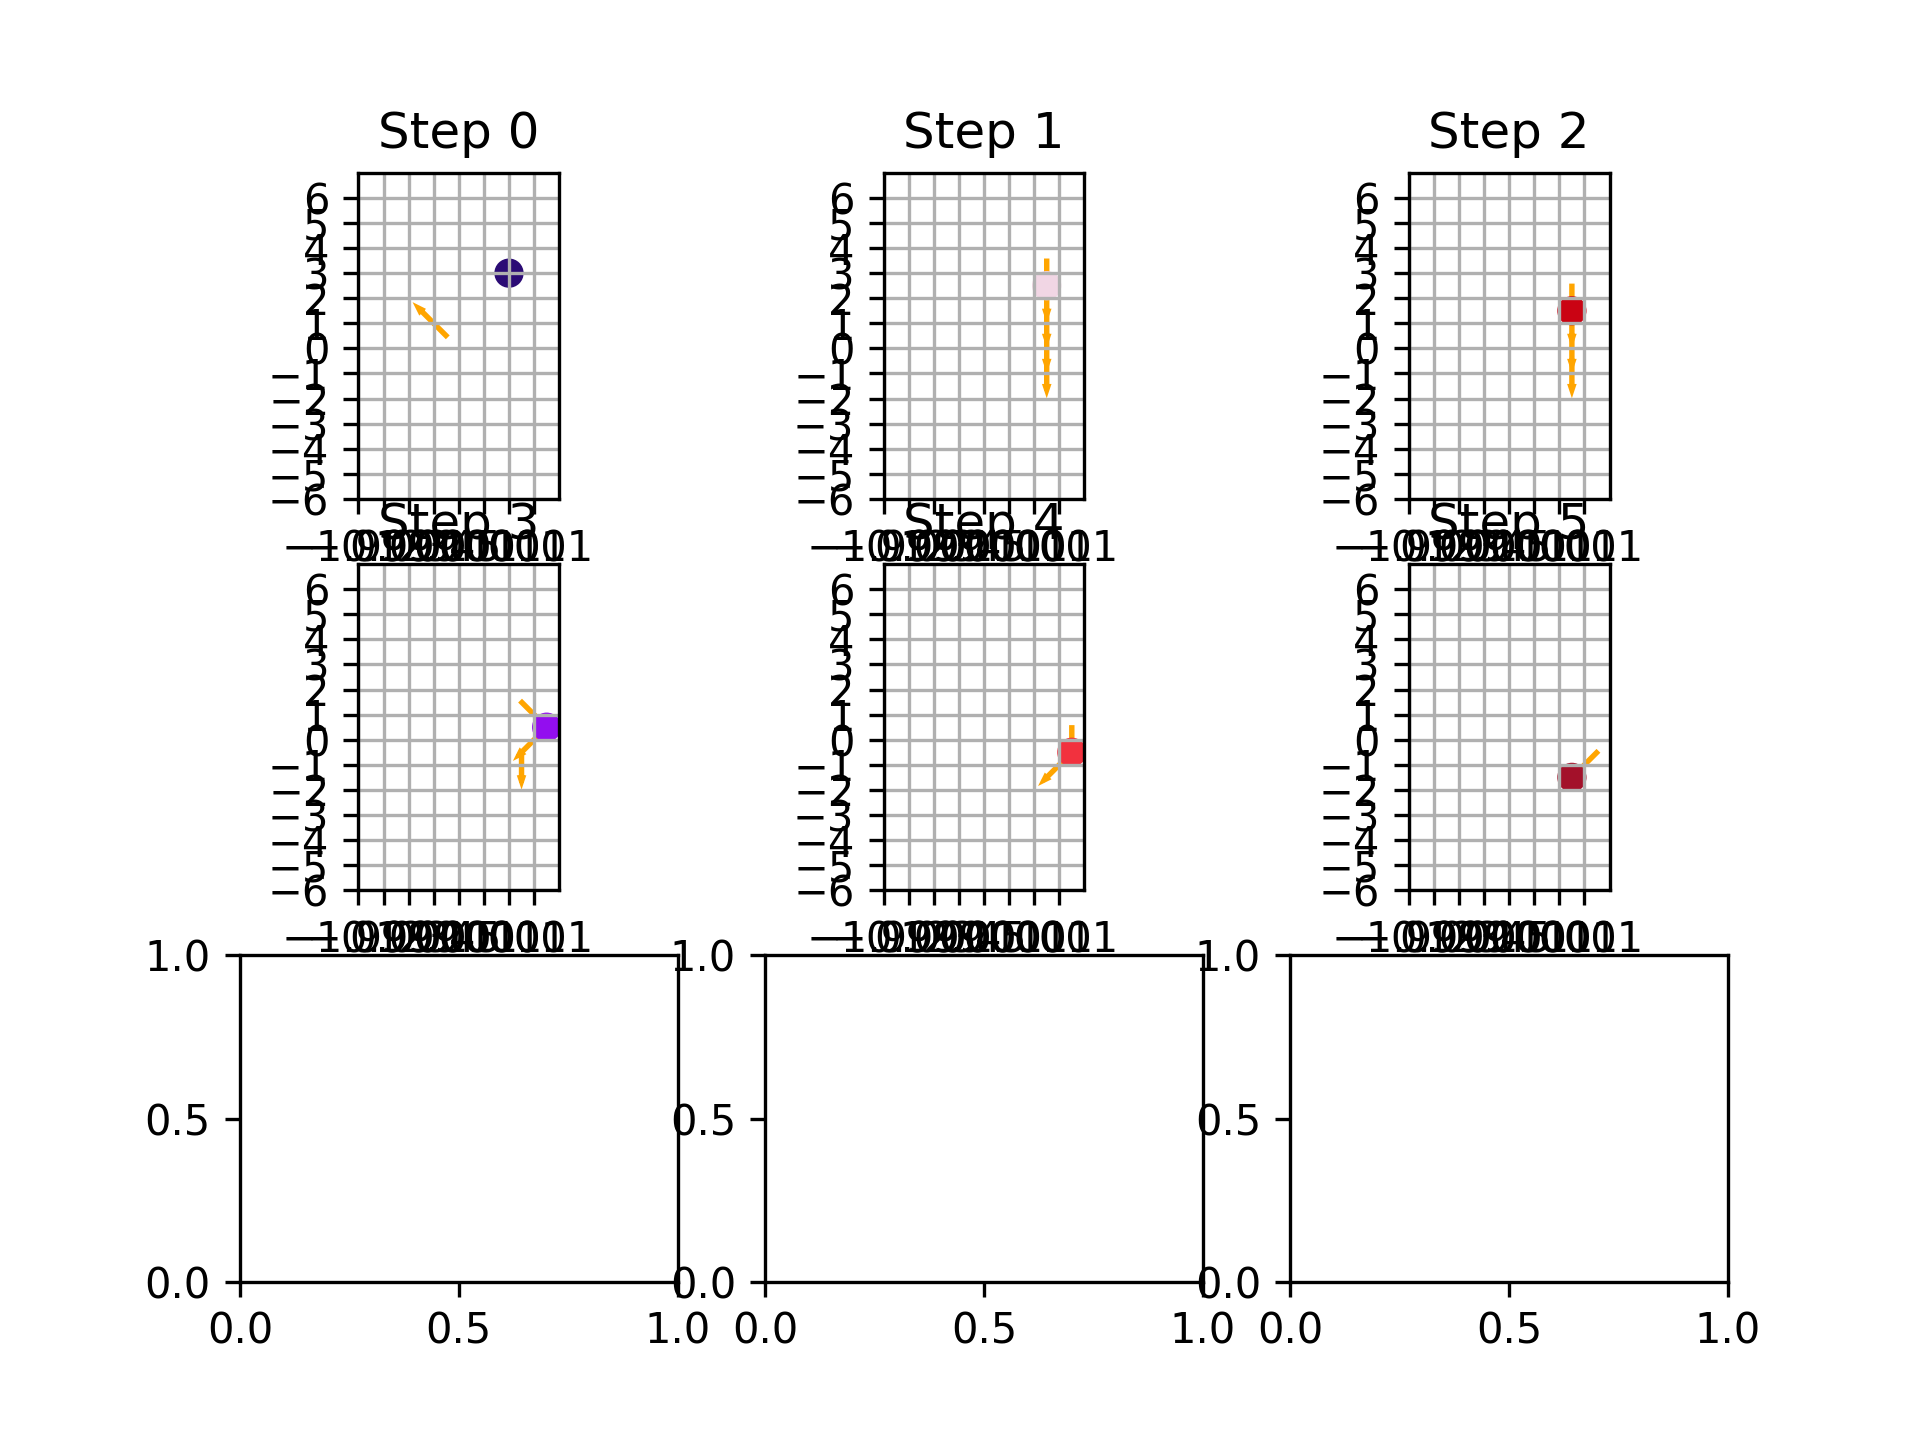
\includegraphics[width=0.4\textwidth]{"outputs/q5: #2.png"}
    \caption{Q5  Plan B.}
\end{figure}

\begin{figure}[H]
    \centering
    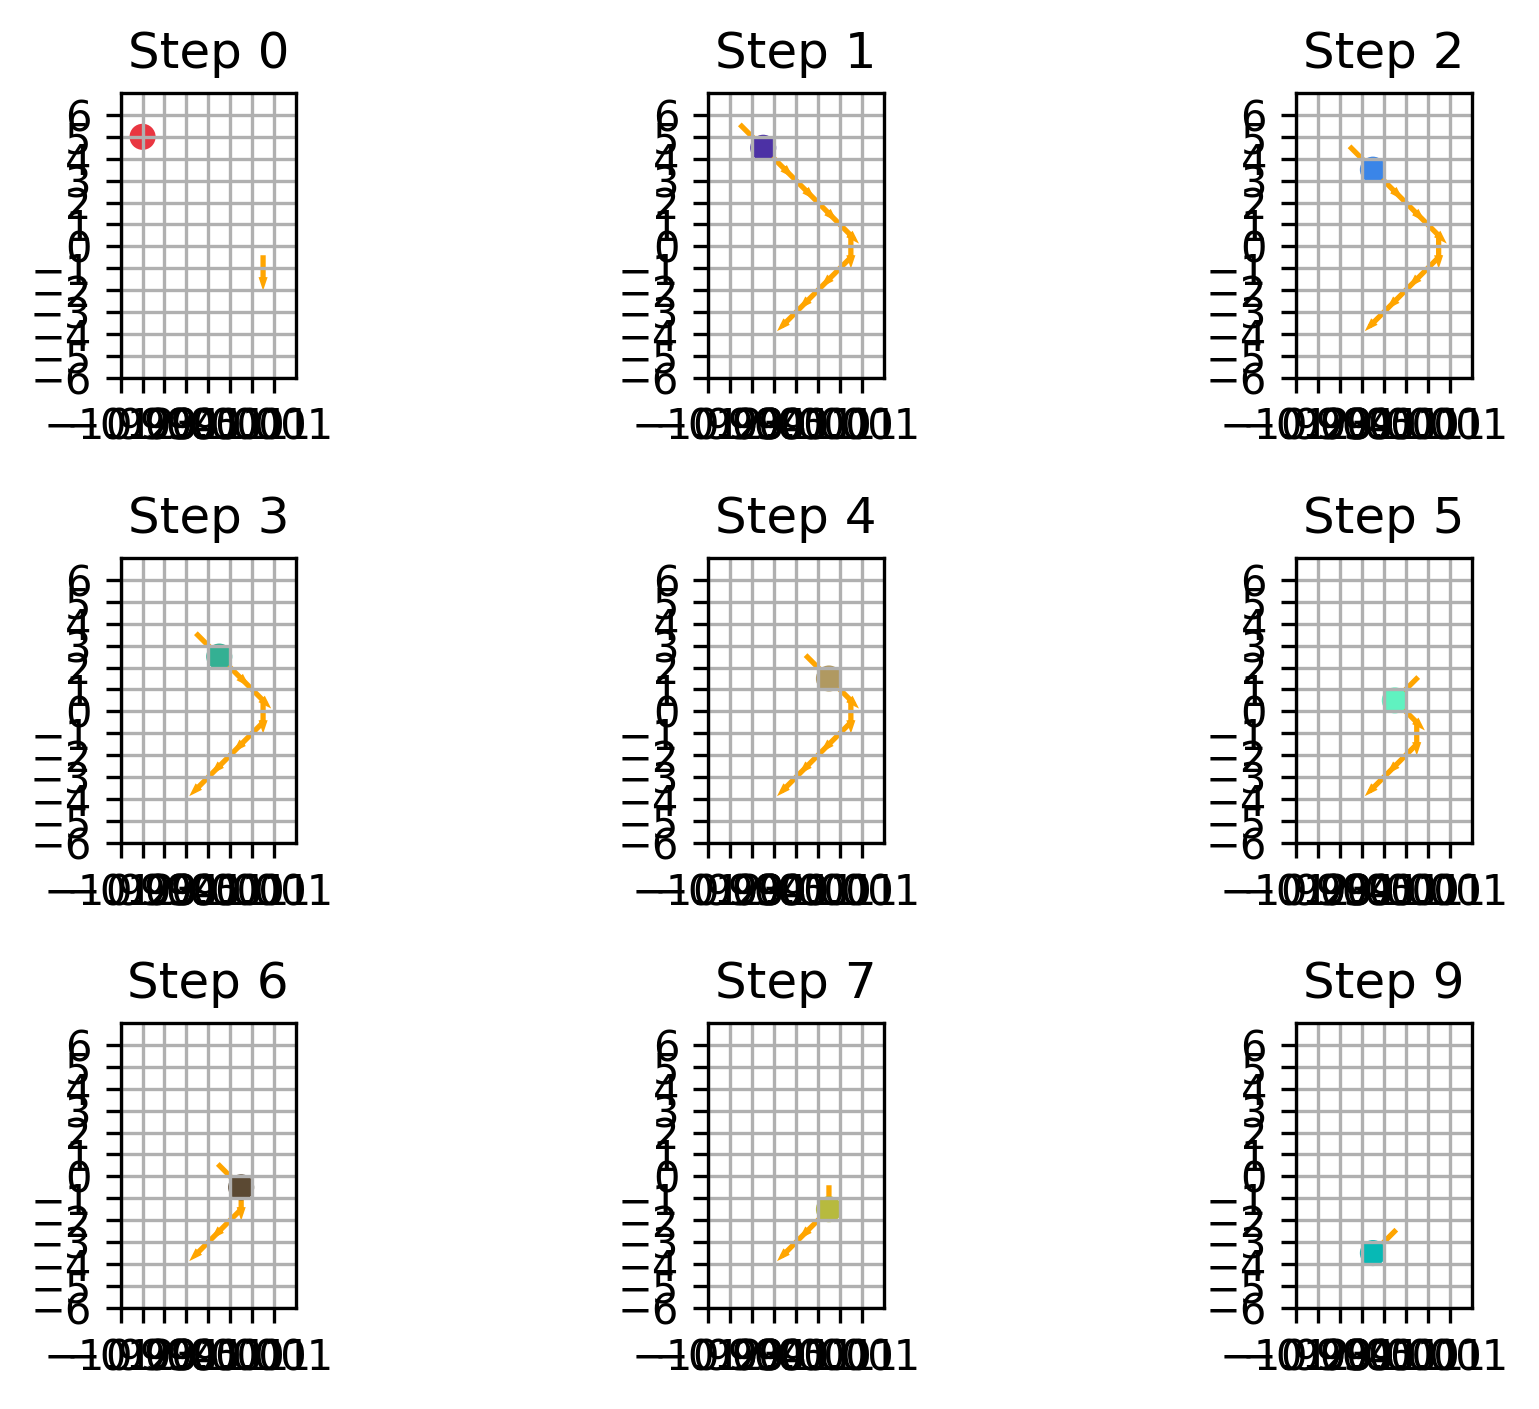
\includegraphics[width=0.4\textwidth]{"outputs/q5: #3.png"}
    \caption{Q5  Plan C.}
\end{figure}

\section{Question 6}
Done. See code.

\section{Question 7}

Because the cost was 1.0 whether A* explored diagonally or straight, it means that the plan will choose diagonal moves that bring it closer to the goal, even if it creates jagged final paths. A simple fix would be to multiply diagonal move's costs by $\sqrt{2}$ to account for the extra distance covered.

\begin{figure}[H]
	\centering
    	\begin{subfigure}{0.33\textwidth}
    		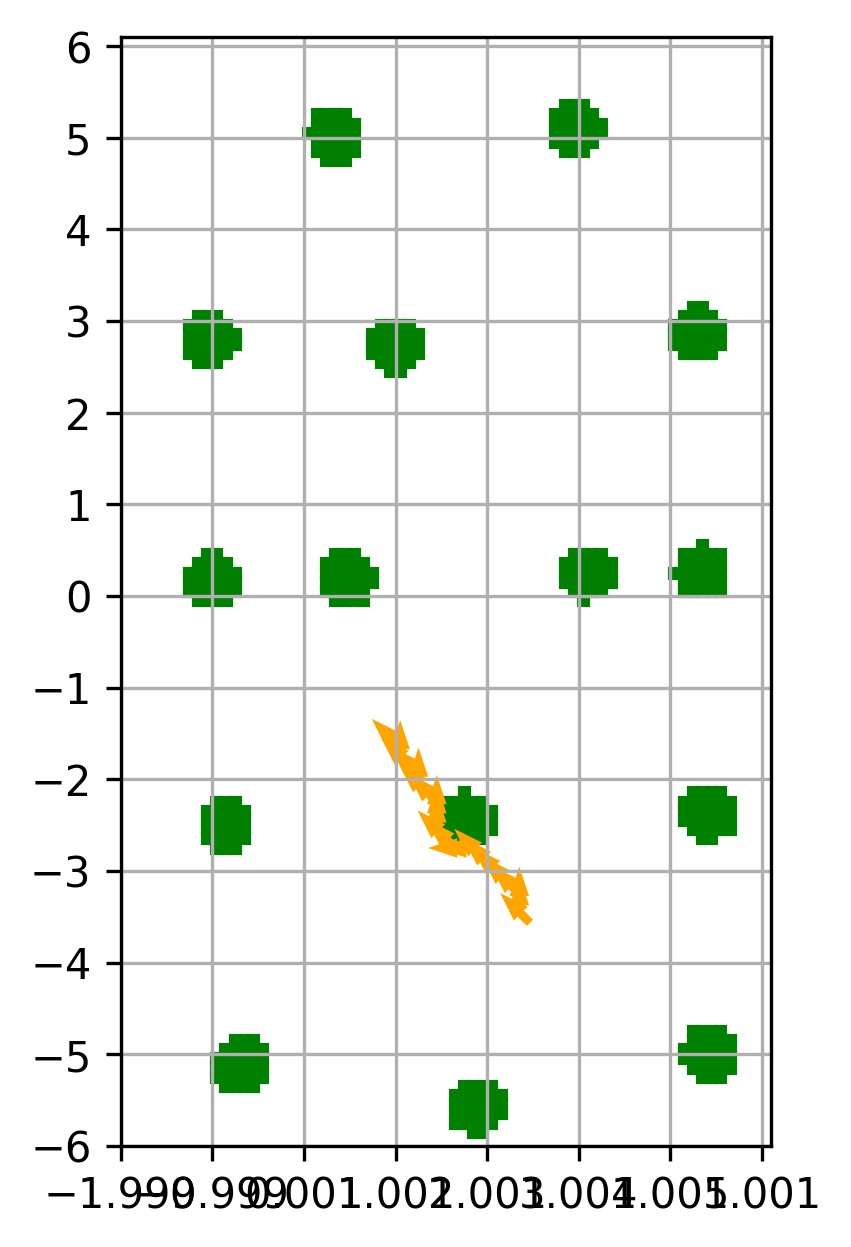
\includegraphics[width=1.0\textwidth]{"outputs/q7: #1.png"}
    		\caption{Q7  Plan A.}
	\end{subfigure}
    	\begin{subfigure}{0.33\textwidth}
    		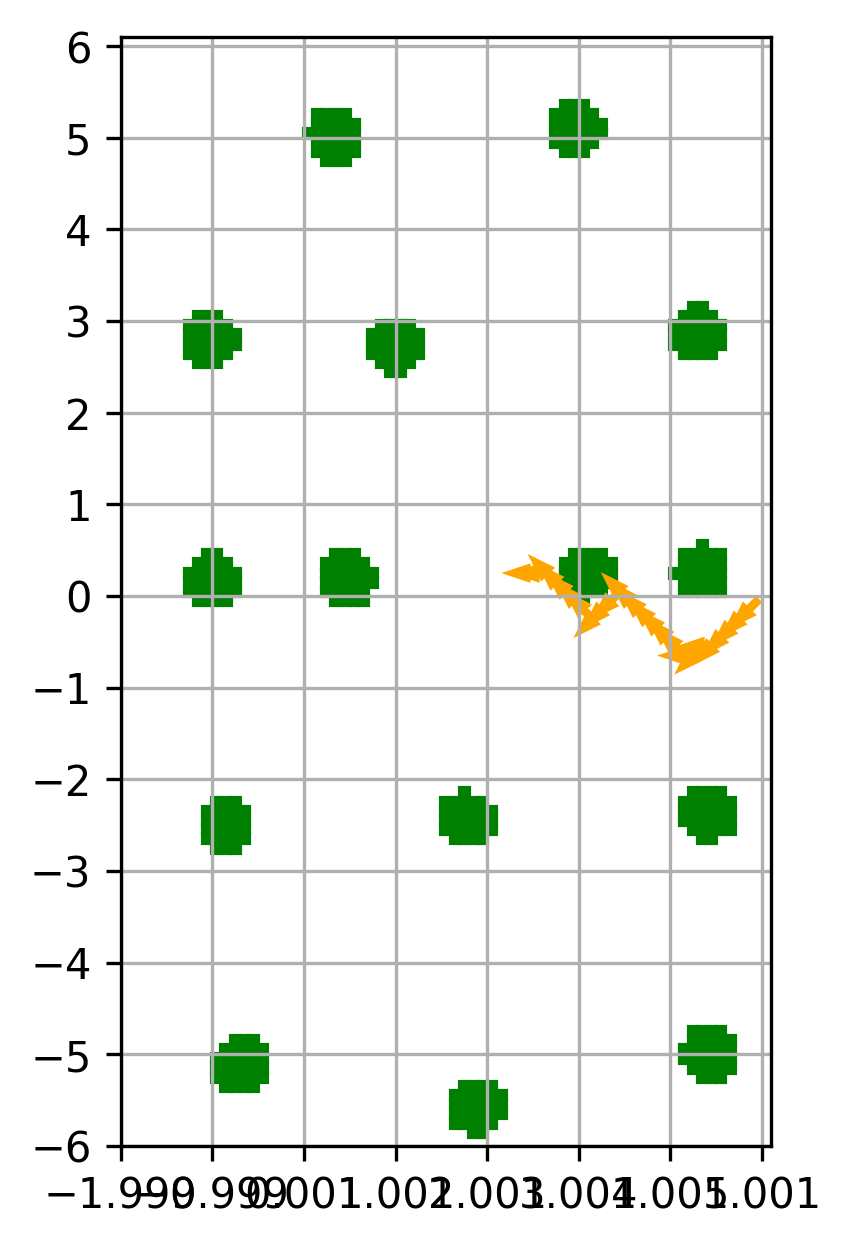
\includegraphics[width=1.0\textwidth]{"outputs/q7: #2.png"}
    		\caption{Q7  Plan B.}
	\end{subfigure}
    	\begin{subfigure}{0.33\textwidth}
    		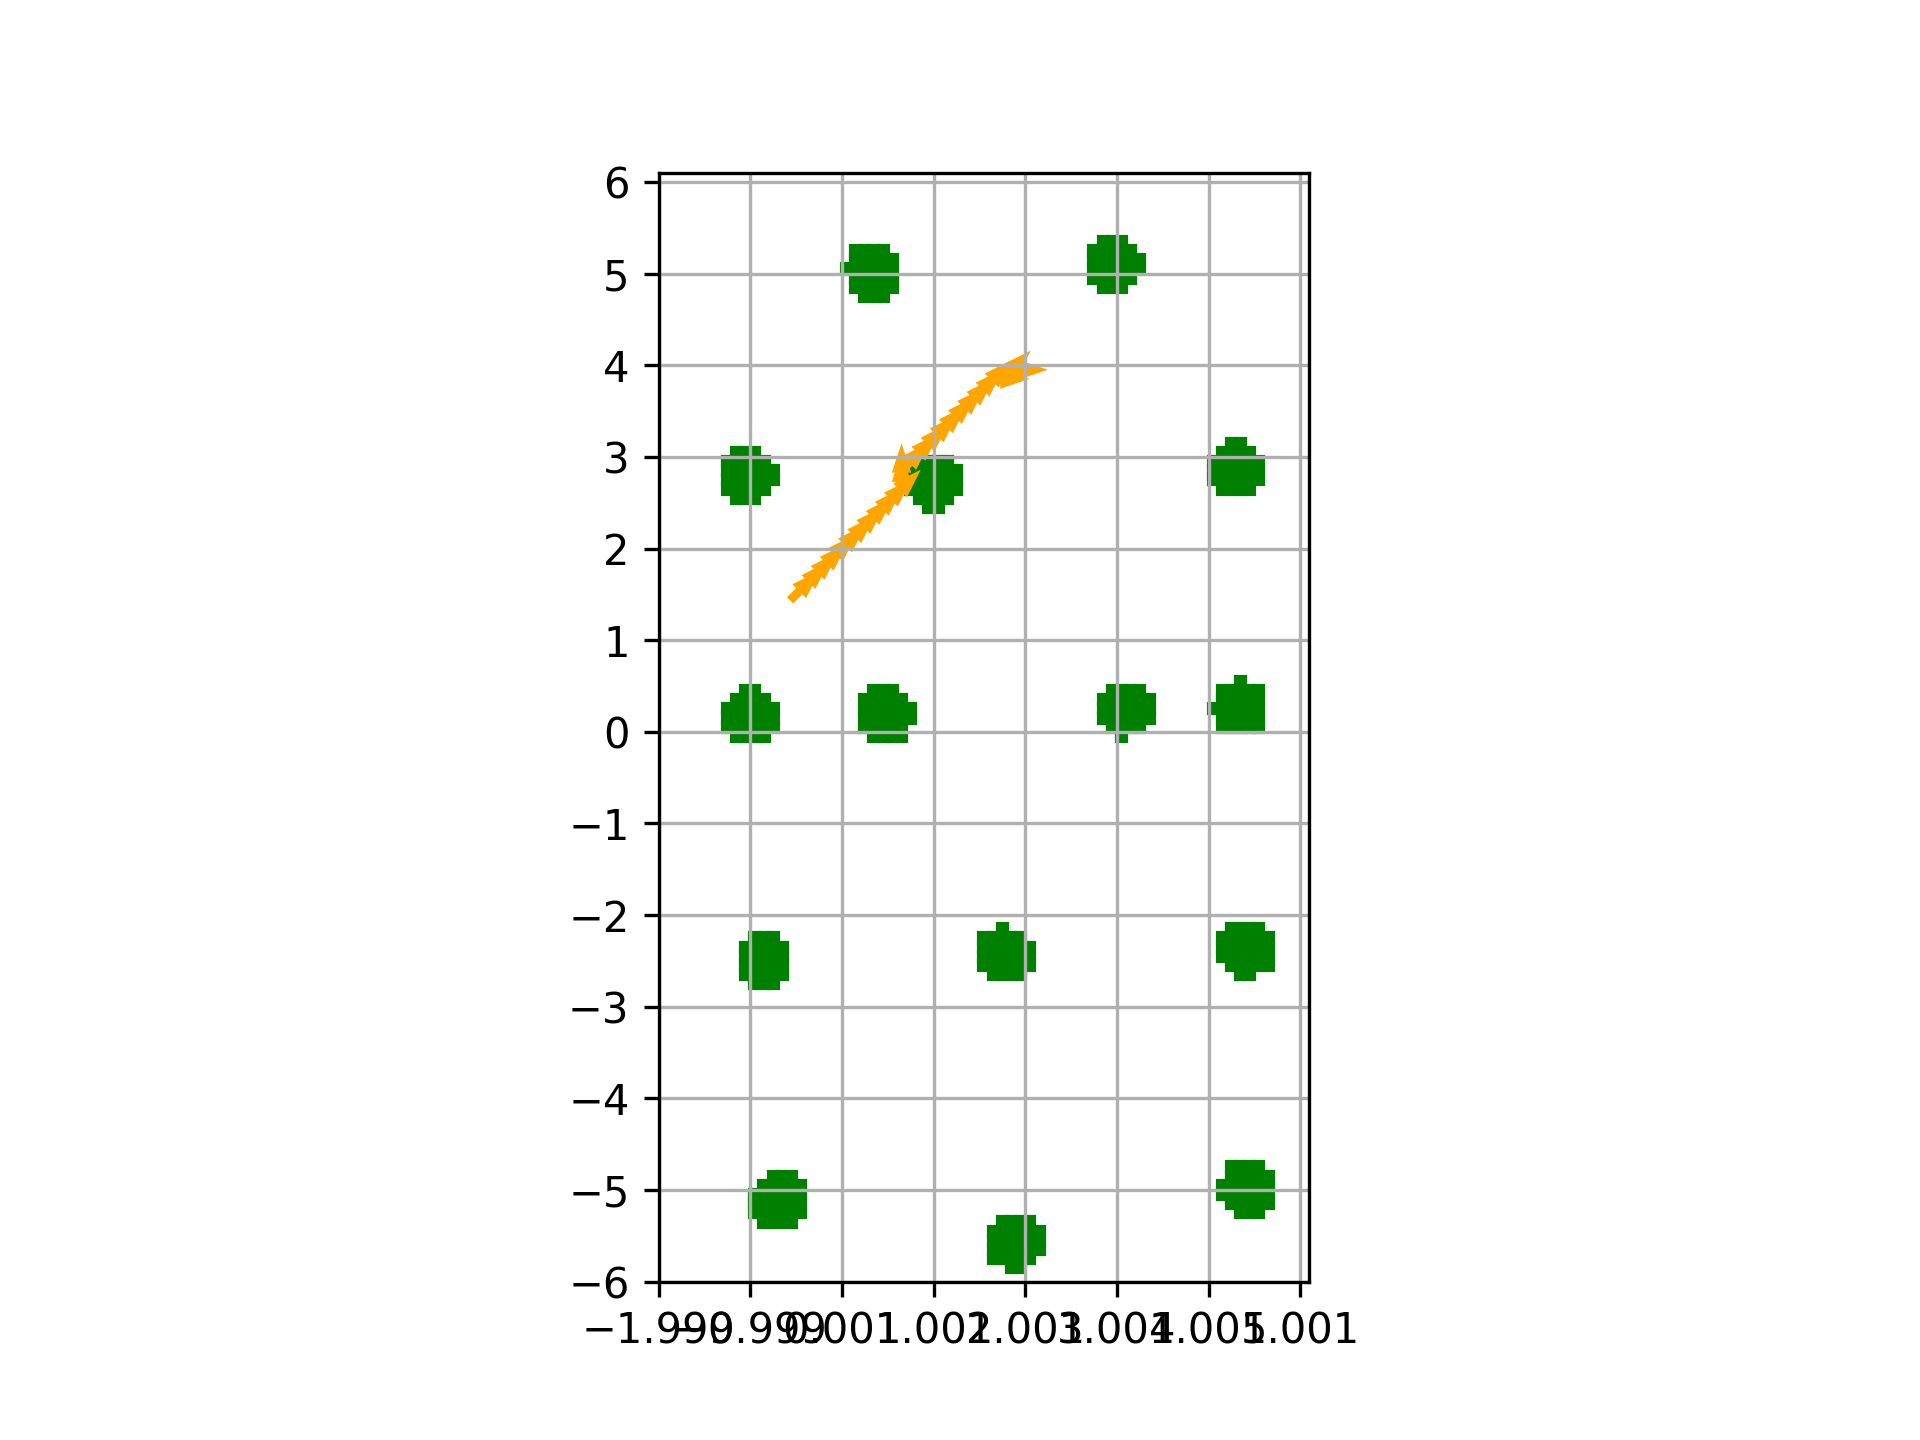
\includegraphics[width=1.0\textwidth]{"outputs/q7: #3.png"}
    		\caption{Q7  Plan C.}
	\end{subfigure}
	
\end{figure}

\section{Question 8}
Done. See code.

I used the state as $(x, y, \theta)$ and the controls as $(v, \omega)$. I use an $\eps$ value of $0.25 * cell_width$ to determine if the robot was near a goal. The $\eps$ value must be less than half the cell-width to ensure the robot only proceeds to the next waypoint cell if it actually entered the previous waypoint cell.

I use my motion model from assignment 0 so refer to that submission for more details on my motion model. I also use my range and bearing calculating equation from assignment 0.

For the controller I use a simple proportional controller based on the error in heading and range. The gains were tuned empirically to 0.5, and 0.5

\begin{equation}
	v_{cmd} = K_v * e_v
\end{equation}

\begin{equation}
	\theta_{cmd} = K_{\theta} * e_{\theta}
\end{equation}

The acceleration limits were enforced by numerically integrating them to velocity limits given the dt value of 0.1.

\begin{equation}
	v_{cmd}' = sign(v_{cmd}) * min(v_{cmd}, v^{\dot}_{max} * dt)
\end{equation}

\section{Question 9}

The robot was able to successfully drive the paths generated in Step 7. Because my controller was proportional only (and not optimally tuned), the robot sometimes overshot the waypoint and had to circle back.

Continuous robot path in purple.
\begin{figure}[H]
	\centering
    	\begin{subfigure}{0.33\textwidth}
    		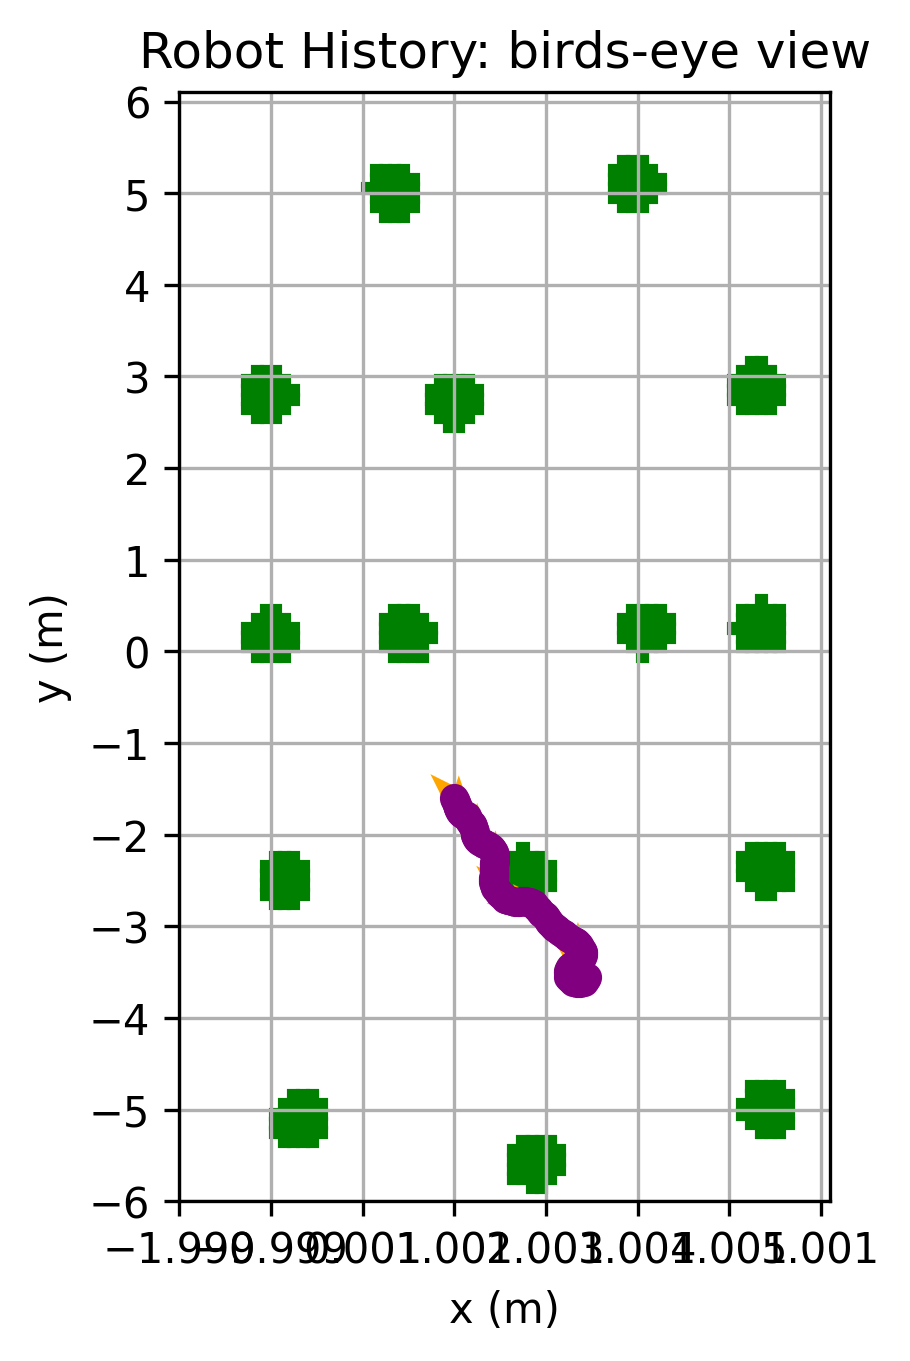
\includegraphics[width=1.0\textwidth]{"outputs/q9: #1.png"}
    		\caption{Q9  Plan 7.A.}
	\end{subfigure}
    	\begin{subfigure}{0.33\textwidth}
    		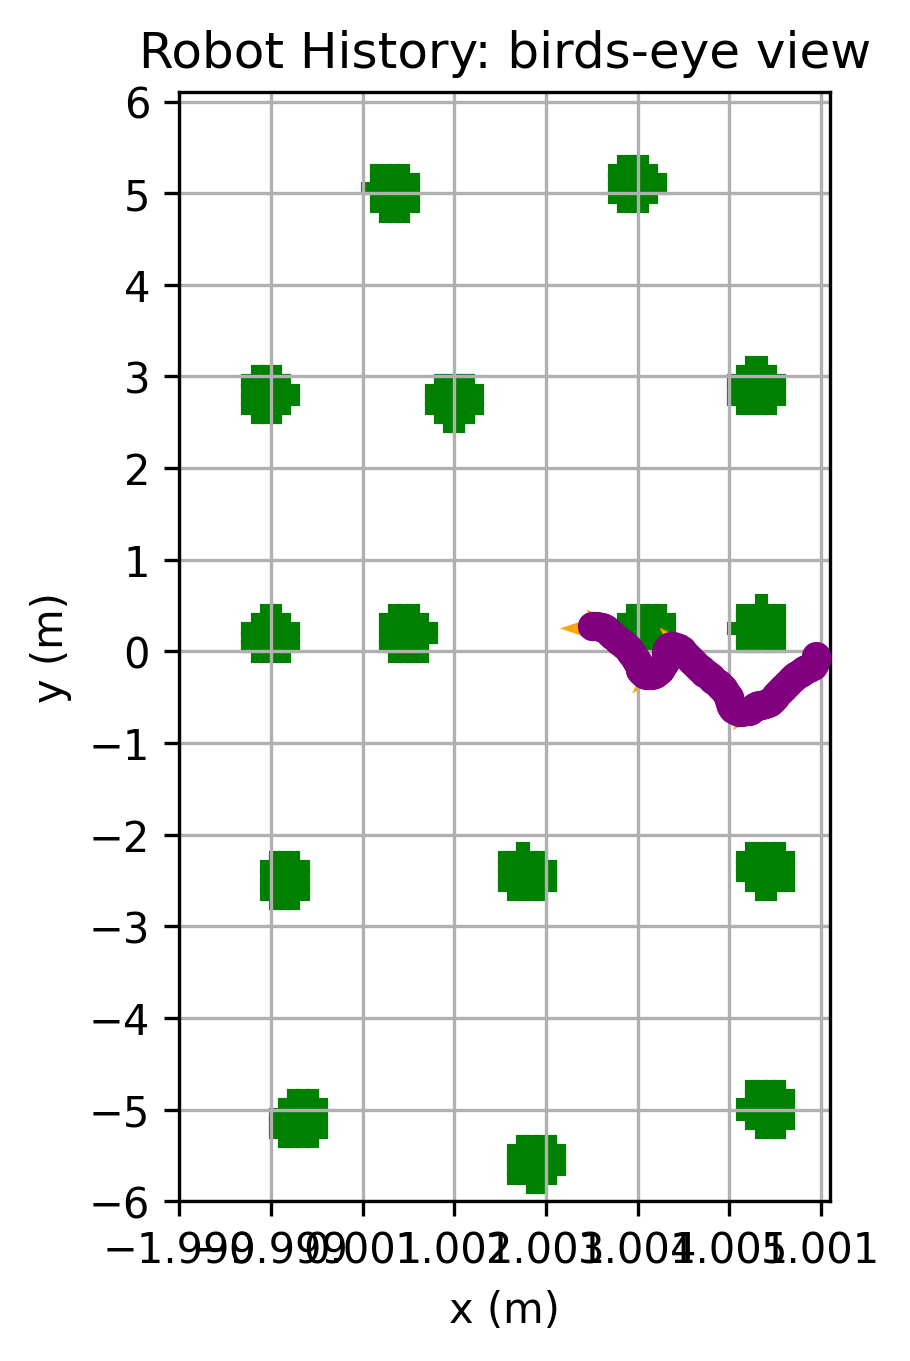
\includegraphics[width=1.0\textwidth]{"outputs/q9: #2.png"}
    		\caption{Q9  Plan 7.B.}
	\end{subfigure}
    	\begin{subfigure}{0.33\textwidth}
    		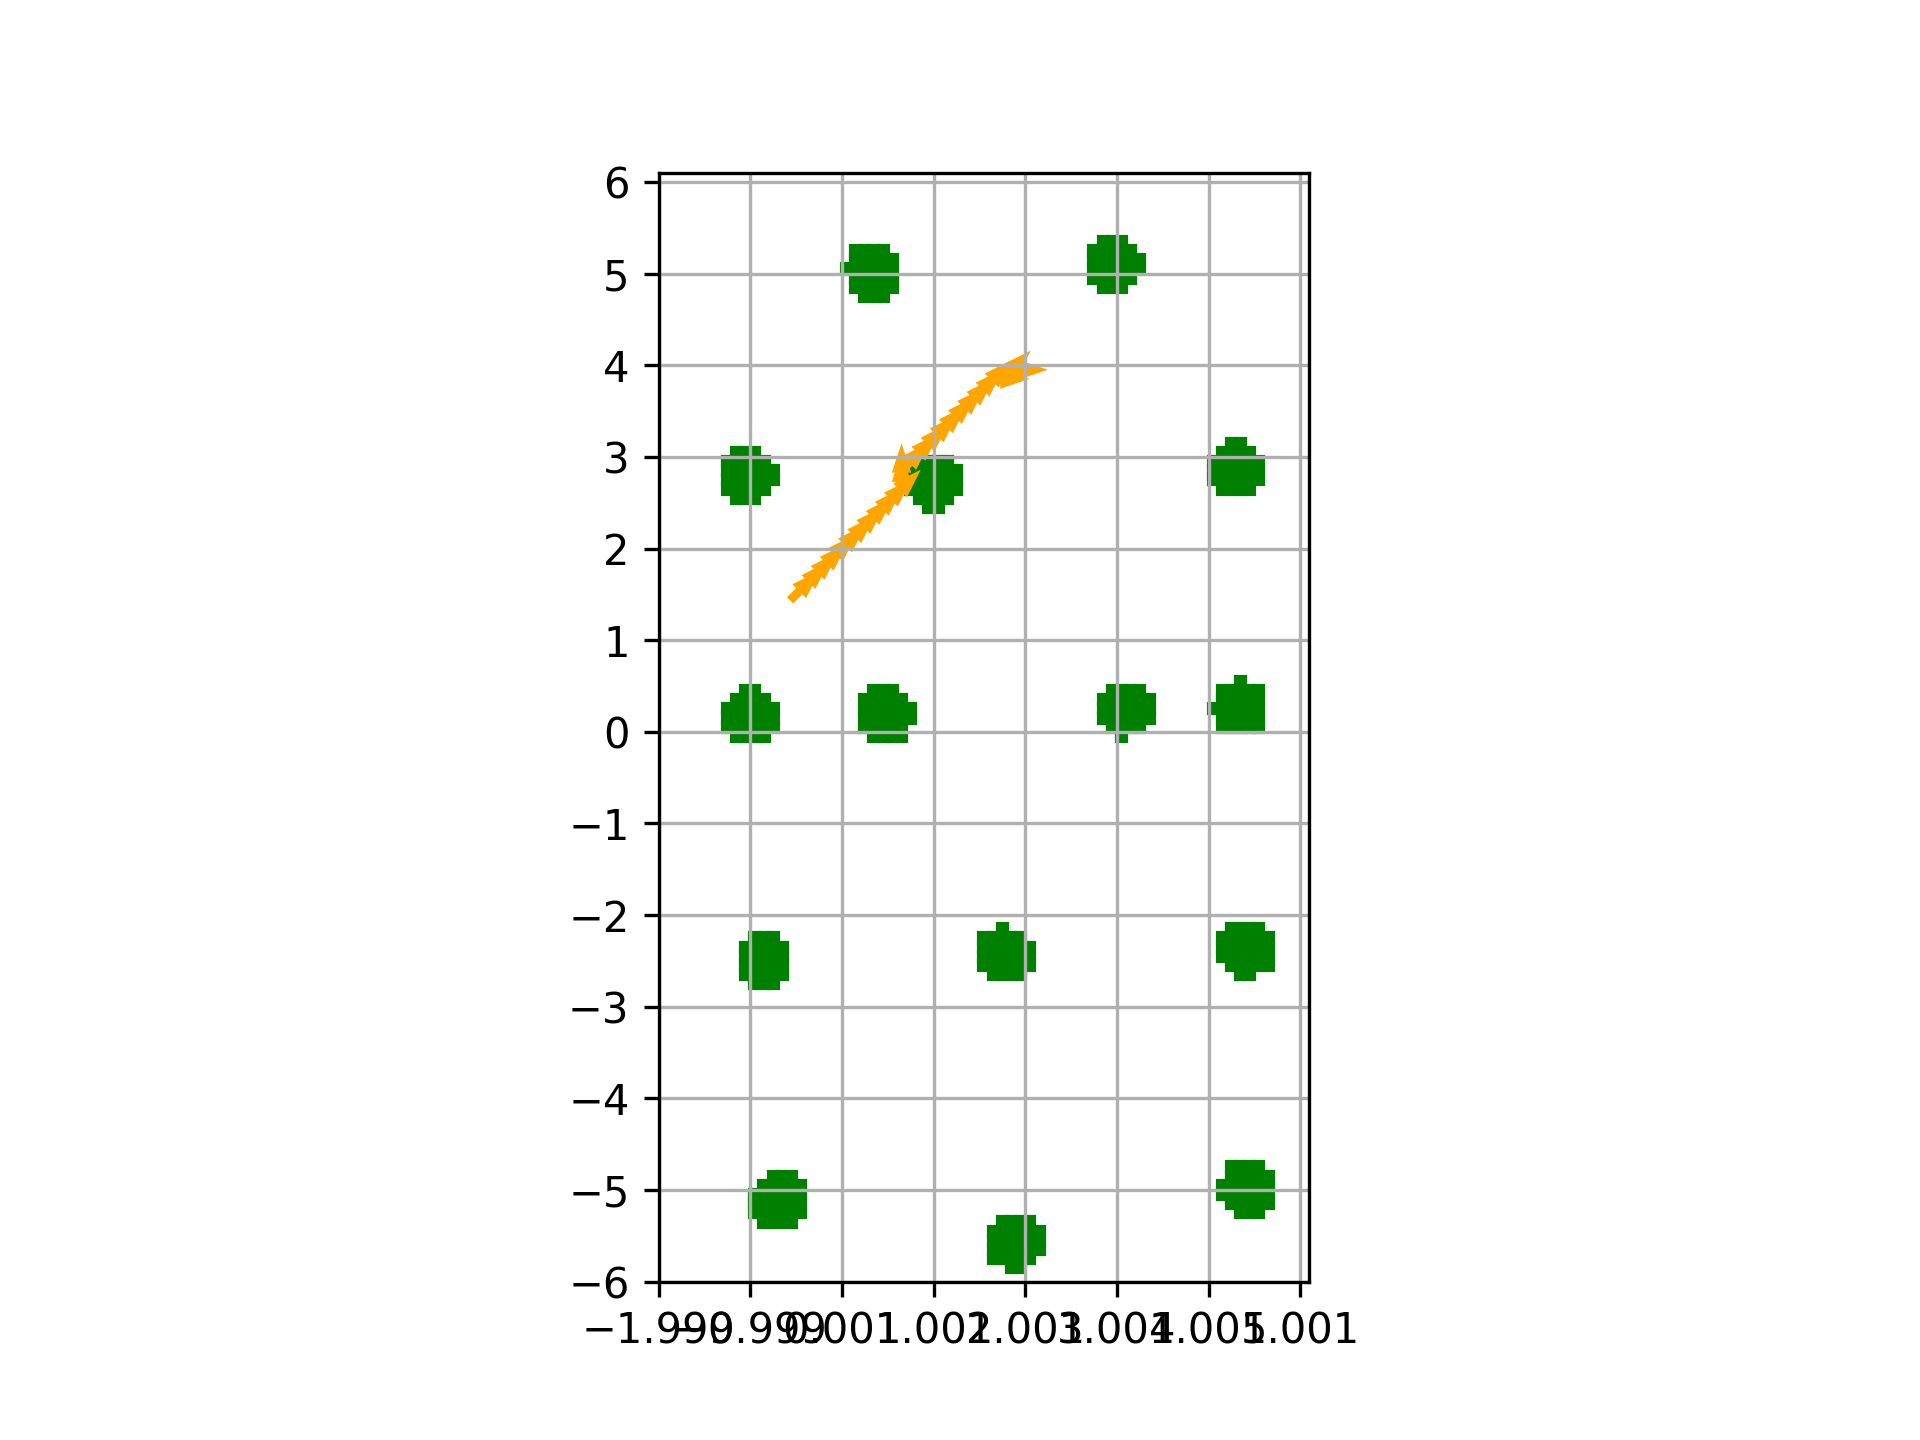
\includegraphics[width=1.0\textwidth]{"outputs/q9: #3.png"}
    		\caption{Q9  Plan 7.C.}
	\end{subfigure}
	
\end{figure}

\section{Question 10}
Because I had already designed my code to be modular and allow both online planners and offline planners, as well as grid robots or continuous robots, it means that programming this step was relatively simple.

Continuous robot path in purple.
\begin{figure}[H]
    \centering
    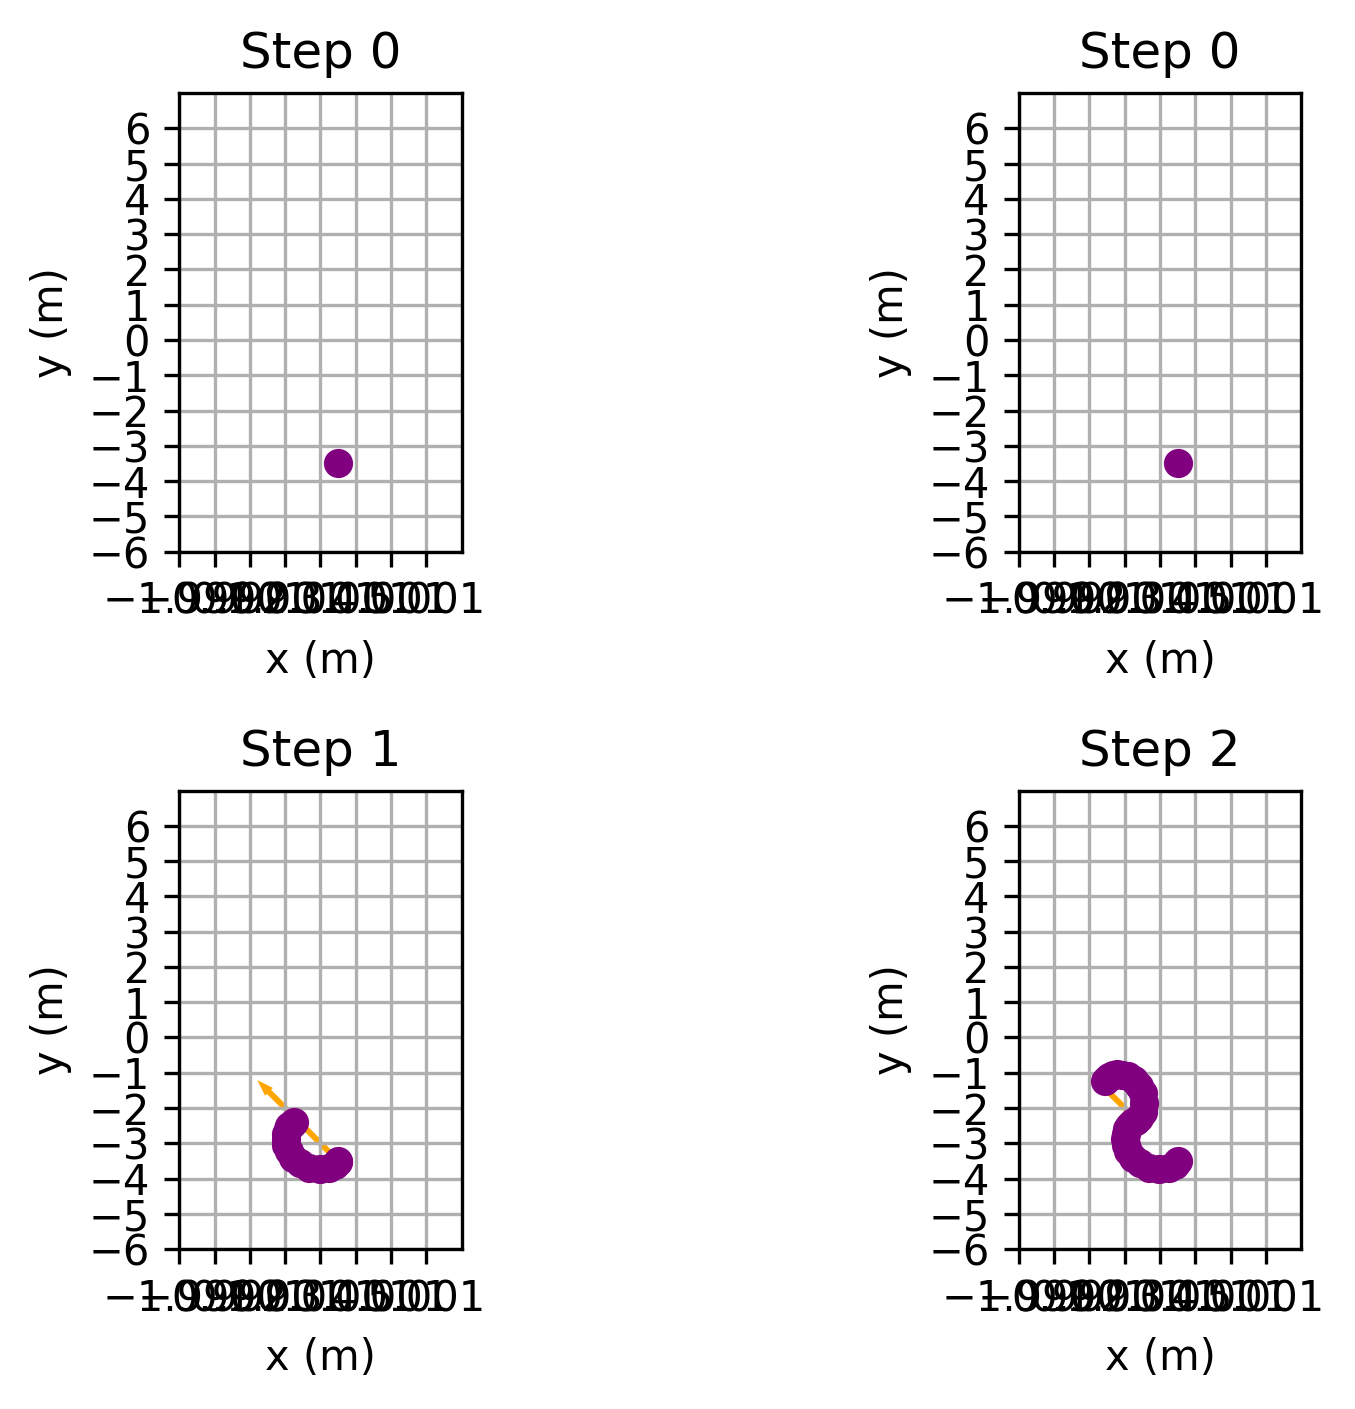
\includegraphics[width=0.4\textwidth]{"outputs/q10: #1.png"}
    \caption{Q10 Online Plan 7.A.}
\end{figure}

\begin{figure}[H]
    \centering
    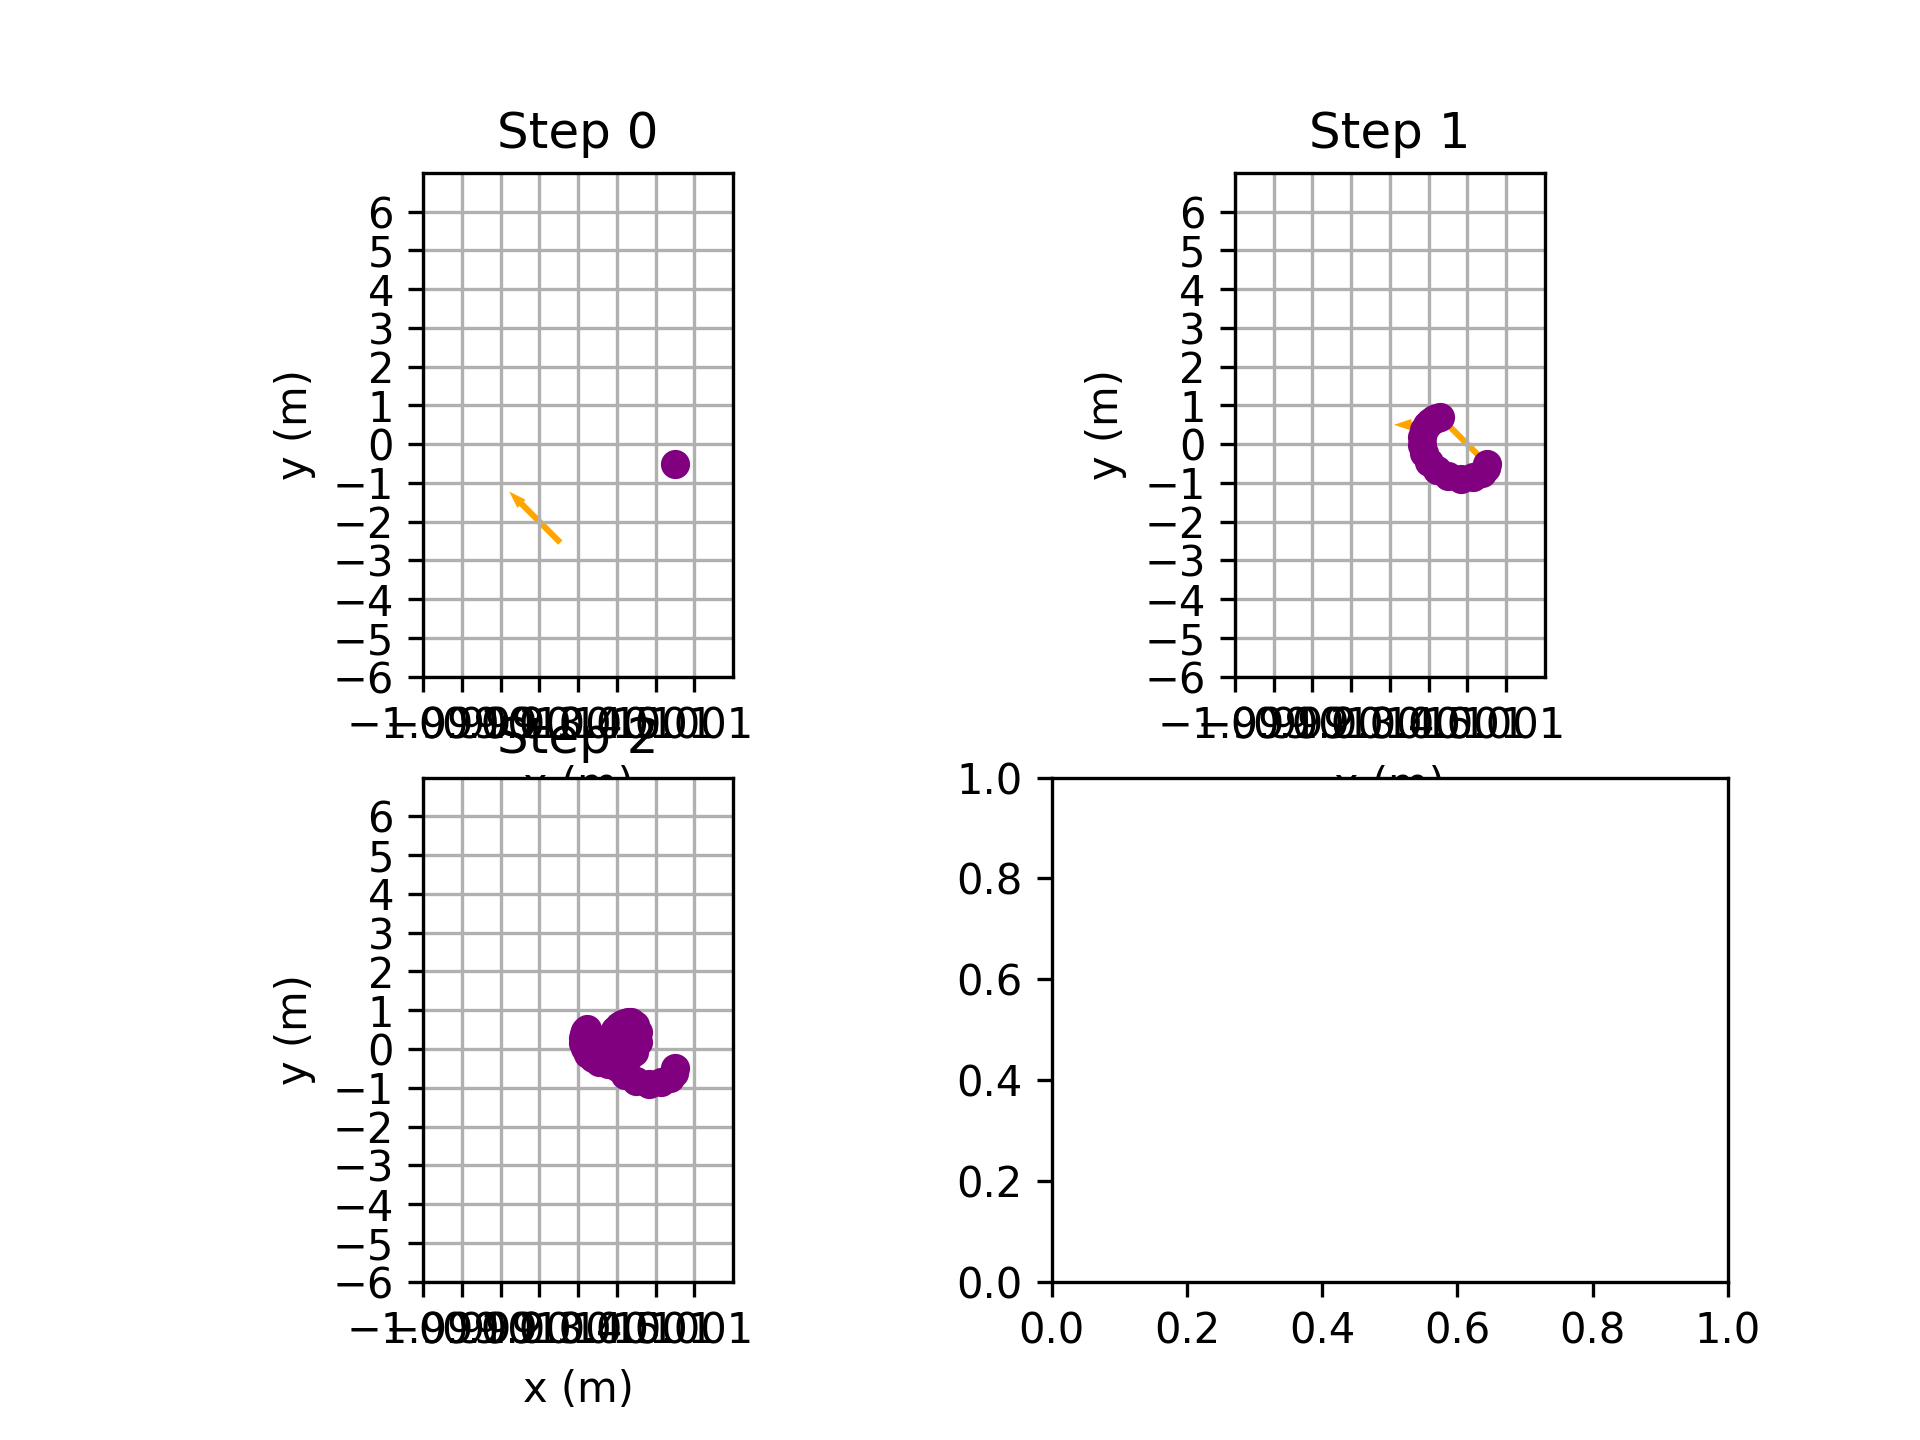
\includegraphics[width=0.4\textwidth]{"outputs/q10: #2.png"}
    \caption{Q10 Online Plan 7.B.}
\end{figure}

\begin{figure}[H]
    \centering
    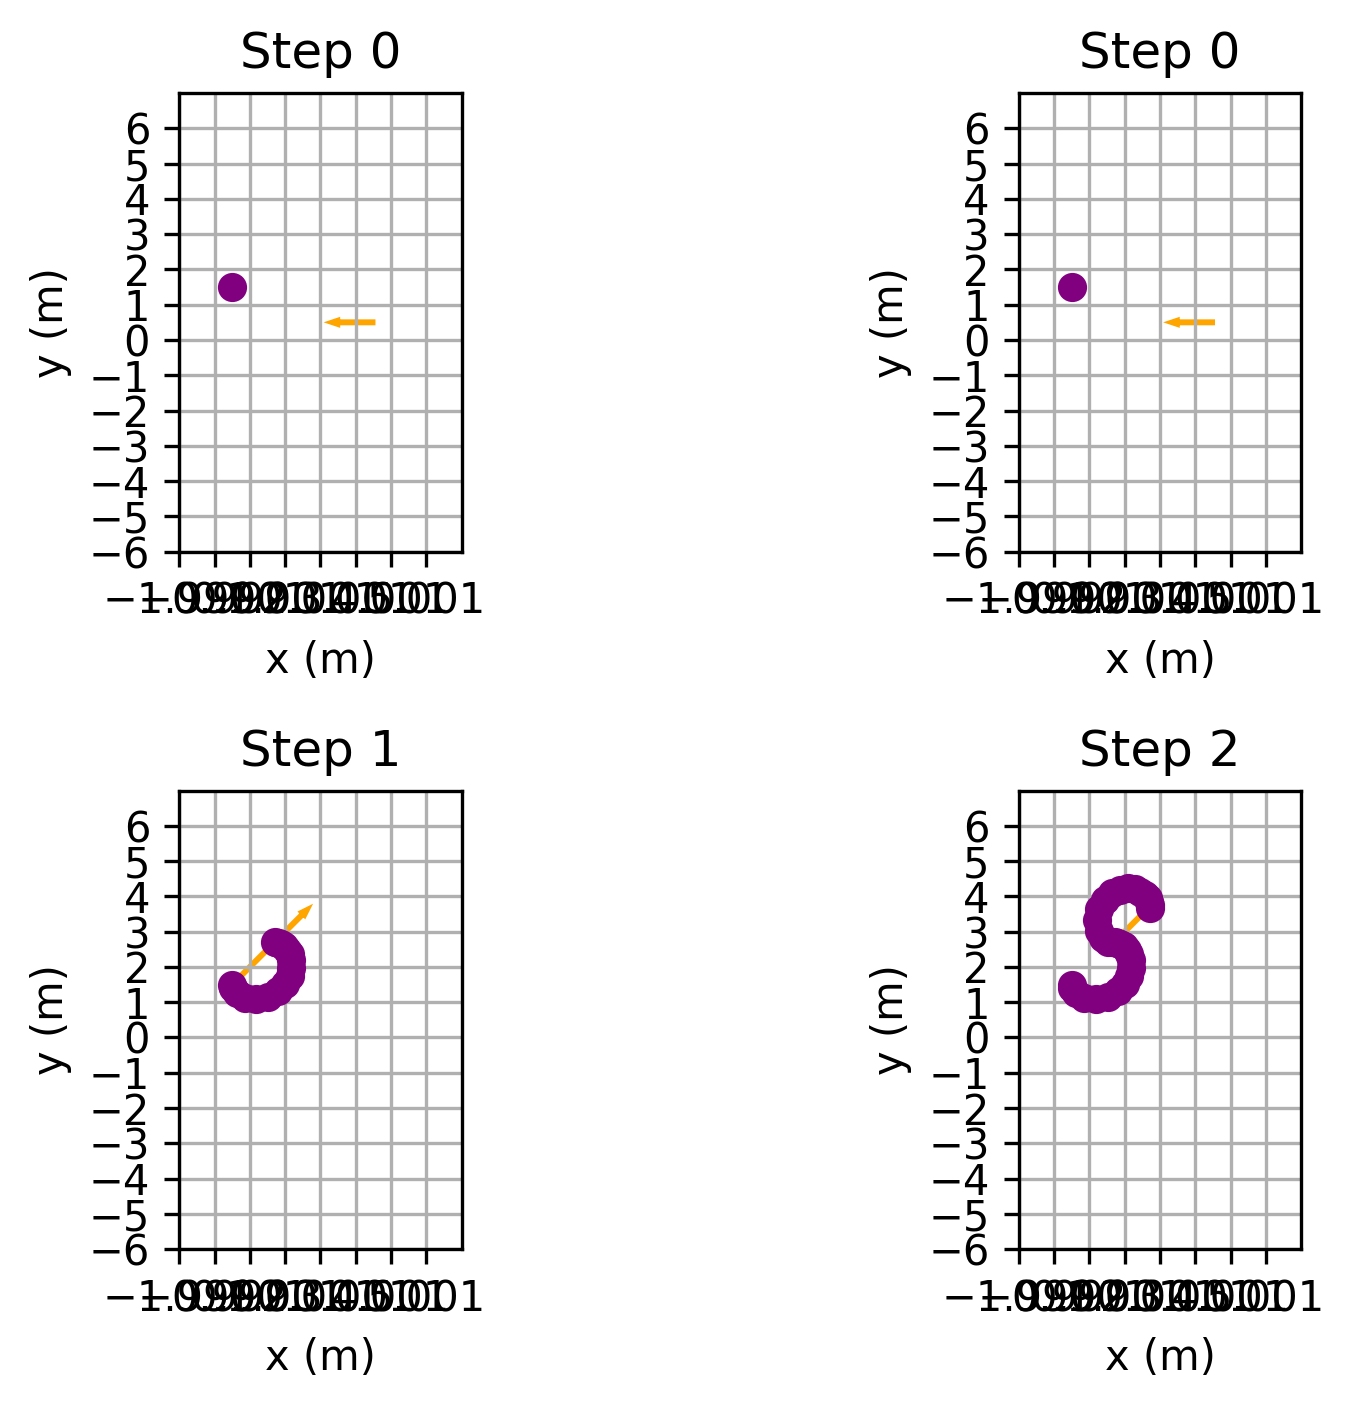
\includegraphics[width=0.4\textwidth]{"outputs/q10: #3.png"}
    \caption{Q10 Online Plan 7.C.}
\end{figure}

\section{Question 11}

Operating on a coarser grid offers some benefits and detriments. First, the planner will complete sooner, meaning that it could be run at a higher frequency during online navigation. But due to the coarseness, it means the final plan won't follow the curvature of obstacles as closely, and therefore will likely take the robot longer to reach its goal.

Finer grids have the opposite properties. They run slower, in fact their computational complexity grows exponentially as the number of state variables increases $O(n^d)$, where n is the number of cells in a dimension, and d is the number of state variables. So increasing the grid density can be extremely costly in higher dimensions.

Finer grids will also yield quicker routes as the plan can skirt more closely around obstacles.

Some coarser grids also yielded curvier continuous robot paths. This may due to the fact that our search space doesn't include heading, which means there's no constraints on what heading the robot has as it drives through waypoints. With my proportional controller, if a goal is far away then it will begin driving more quickly, meaning the radius of curvature will be larger, resulting in the seen curvy paths. This can be corrected by either reducing the $K_v$ value, or by including bearing in the search space, or by using a more complex controller which takes advantage of the robot's holonomic dynamics (ex: zero forward velocity until bearing is perfectly aligned).

Online paths with a grid-width of 1.0

Continuous robot path in purple.
\begin{figure}[H]
    \centering
    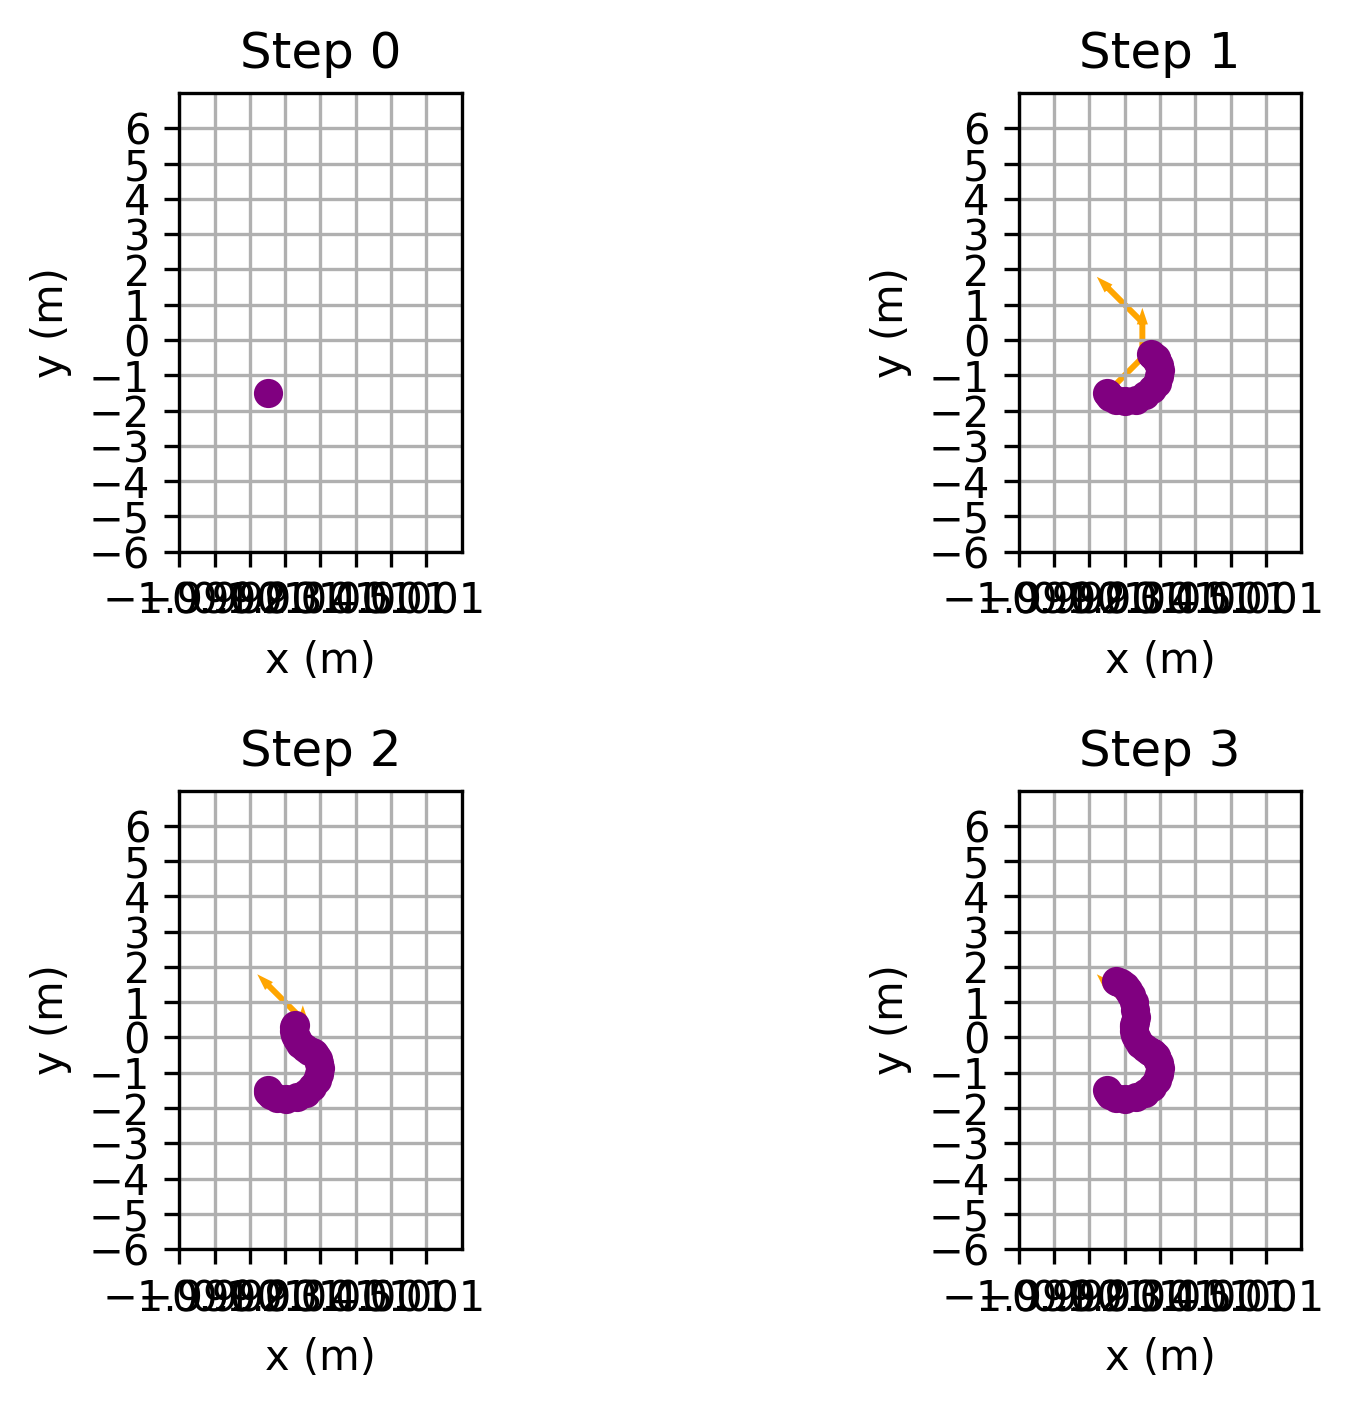
\includegraphics[width=0.4\textwidth]{"outputs/q11: #1.png"}
    \caption{Q11 Online Plan 3.A, cell-width 1.0.}
\end{figure}

\begin{figure}[H]
    \centering
    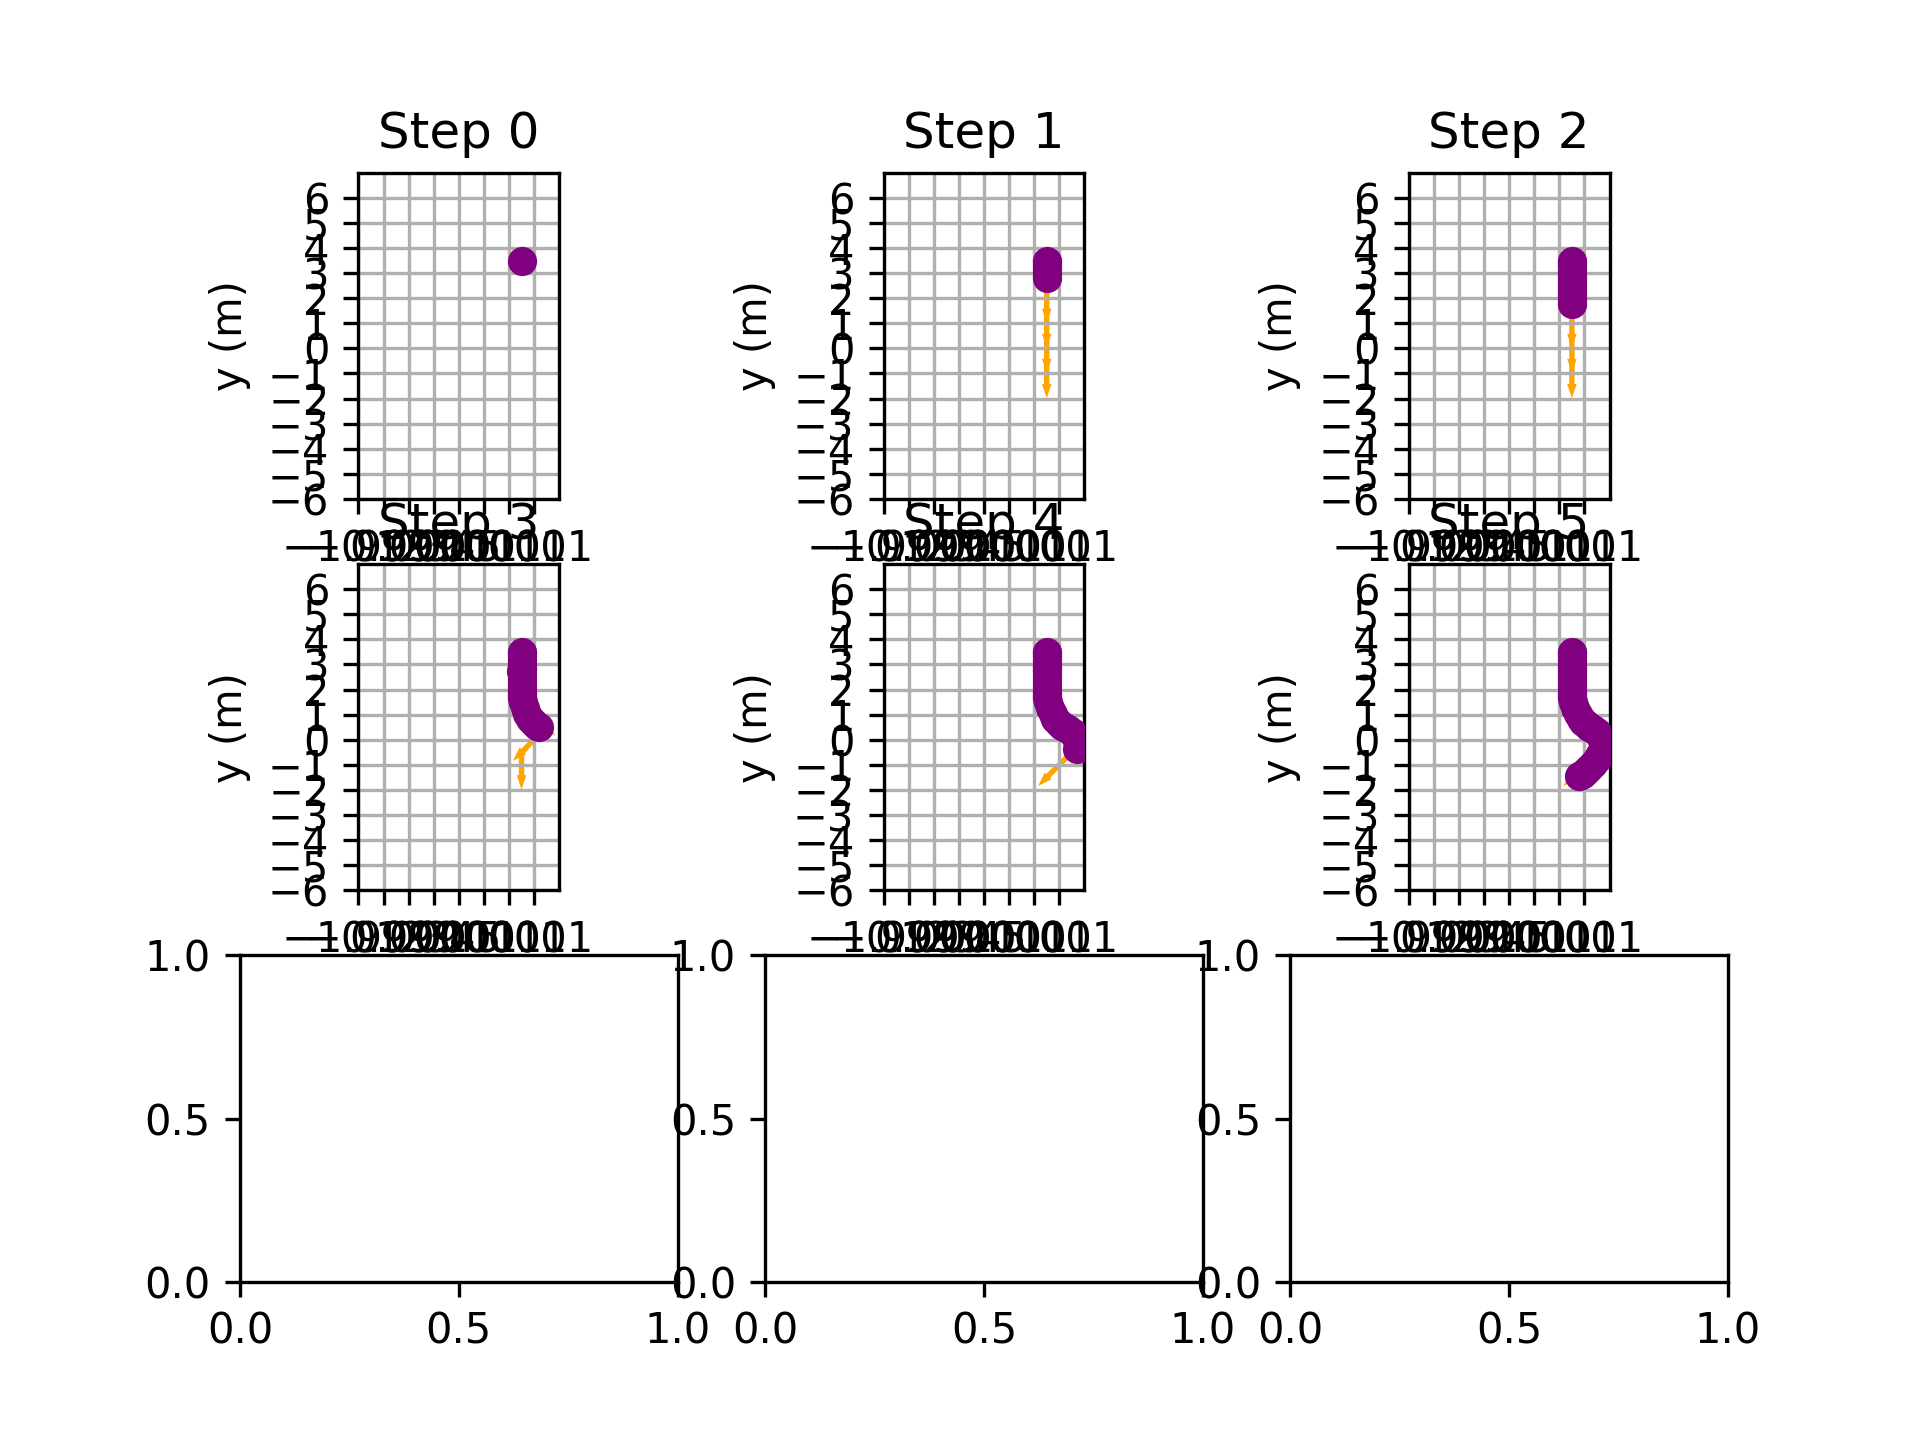
\includegraphics[width=0.4\textwidth]{"outputs/q11: #2.png"}
    \caption{Q11 Online Plan 3.B, cell-width 1.0.}
\end{figure}

\begin{figure}[H]
    \centering
    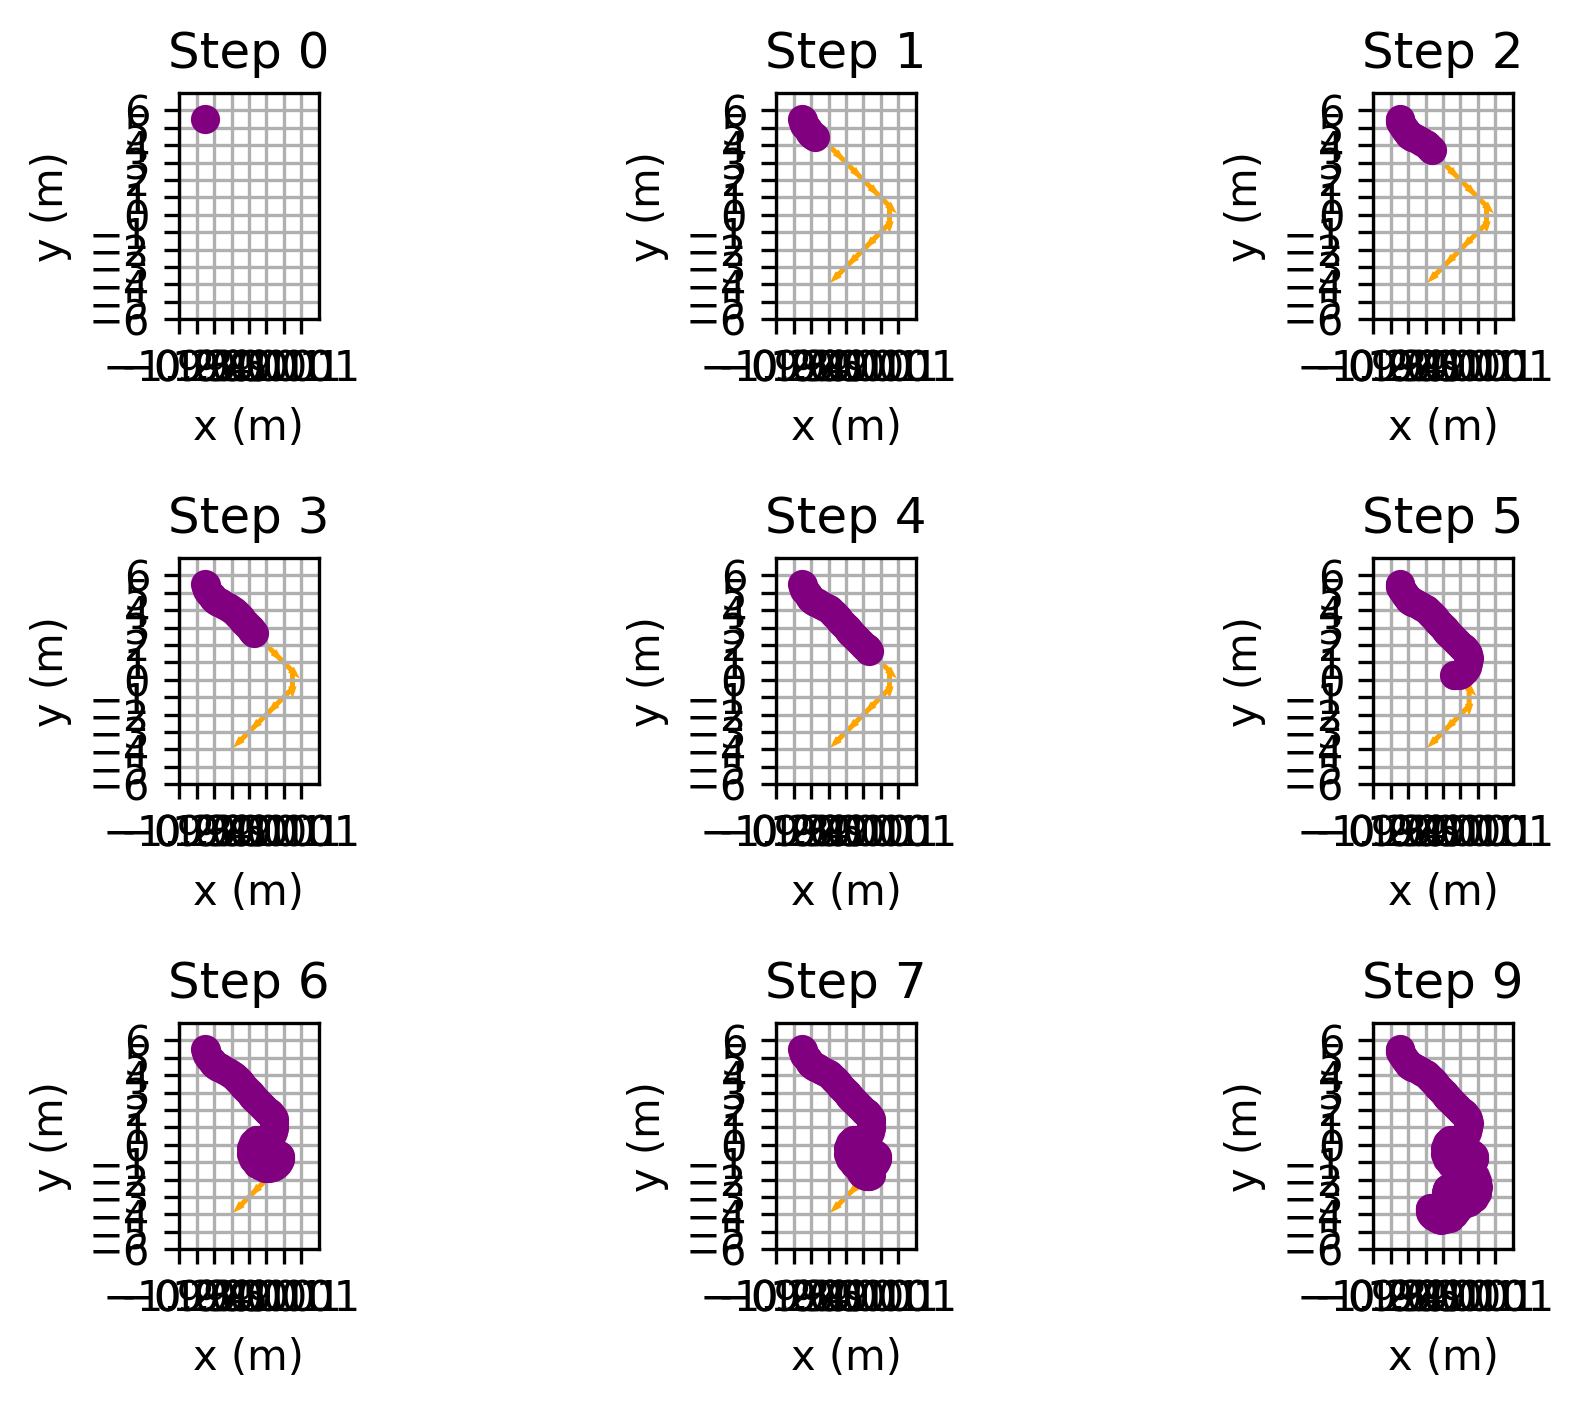
\includegraphics[width=0.5\textwidth]{"outputs/q11: #3.png"}
    \caption{Q11 Online Plan 3.C, cell-width 1.0.}
\end{figure}


Online paths with a grid-width of 0.1:

Continuous robot path in purple.
\begin{figure}[H]
    \centering
    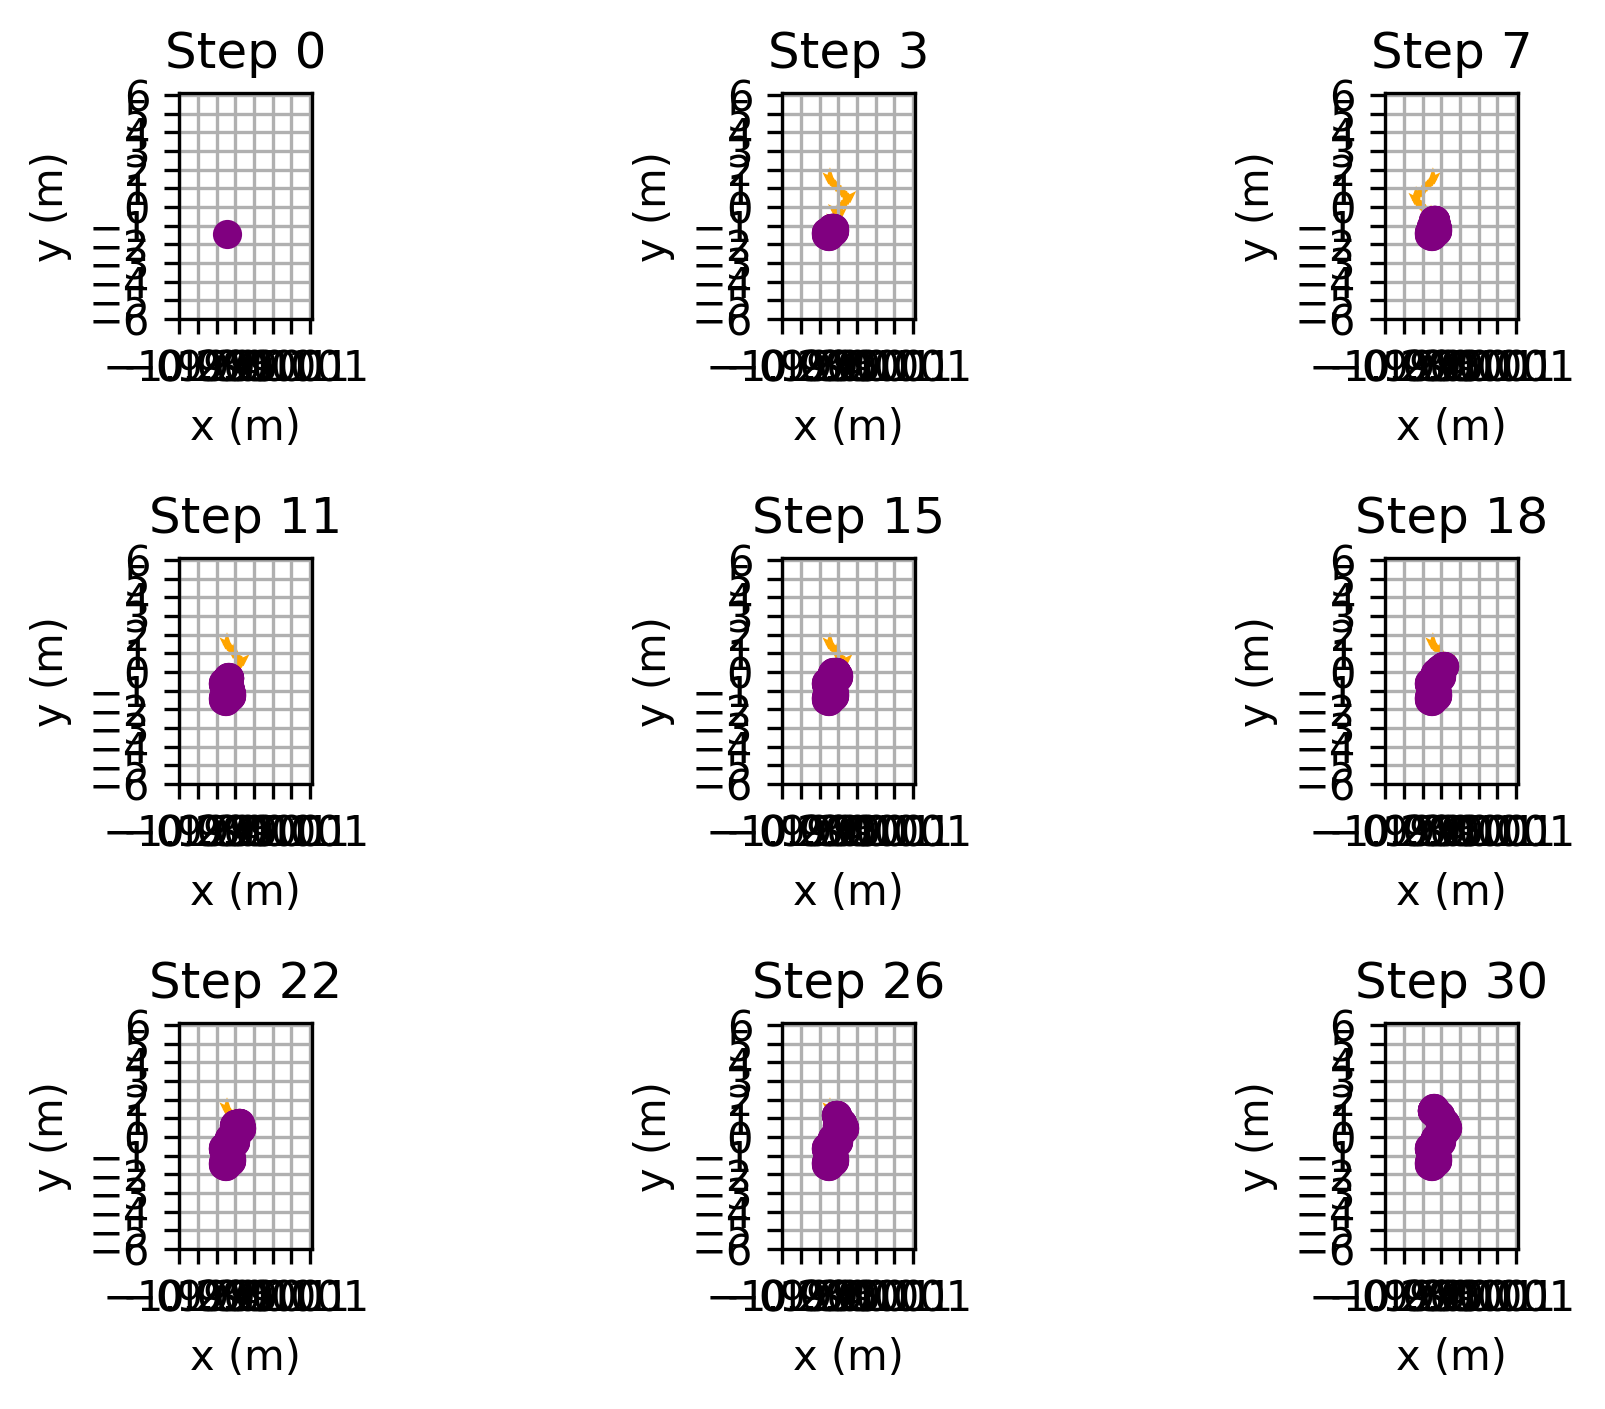
\includegraphics[width=0.4\textwidth]{"outputs/q11: #4.png"}
    \caption{Q11 Online Plan 3.A, cell-width 0.1}
\end{figure}


\begin{figure}[H]
    \centering
    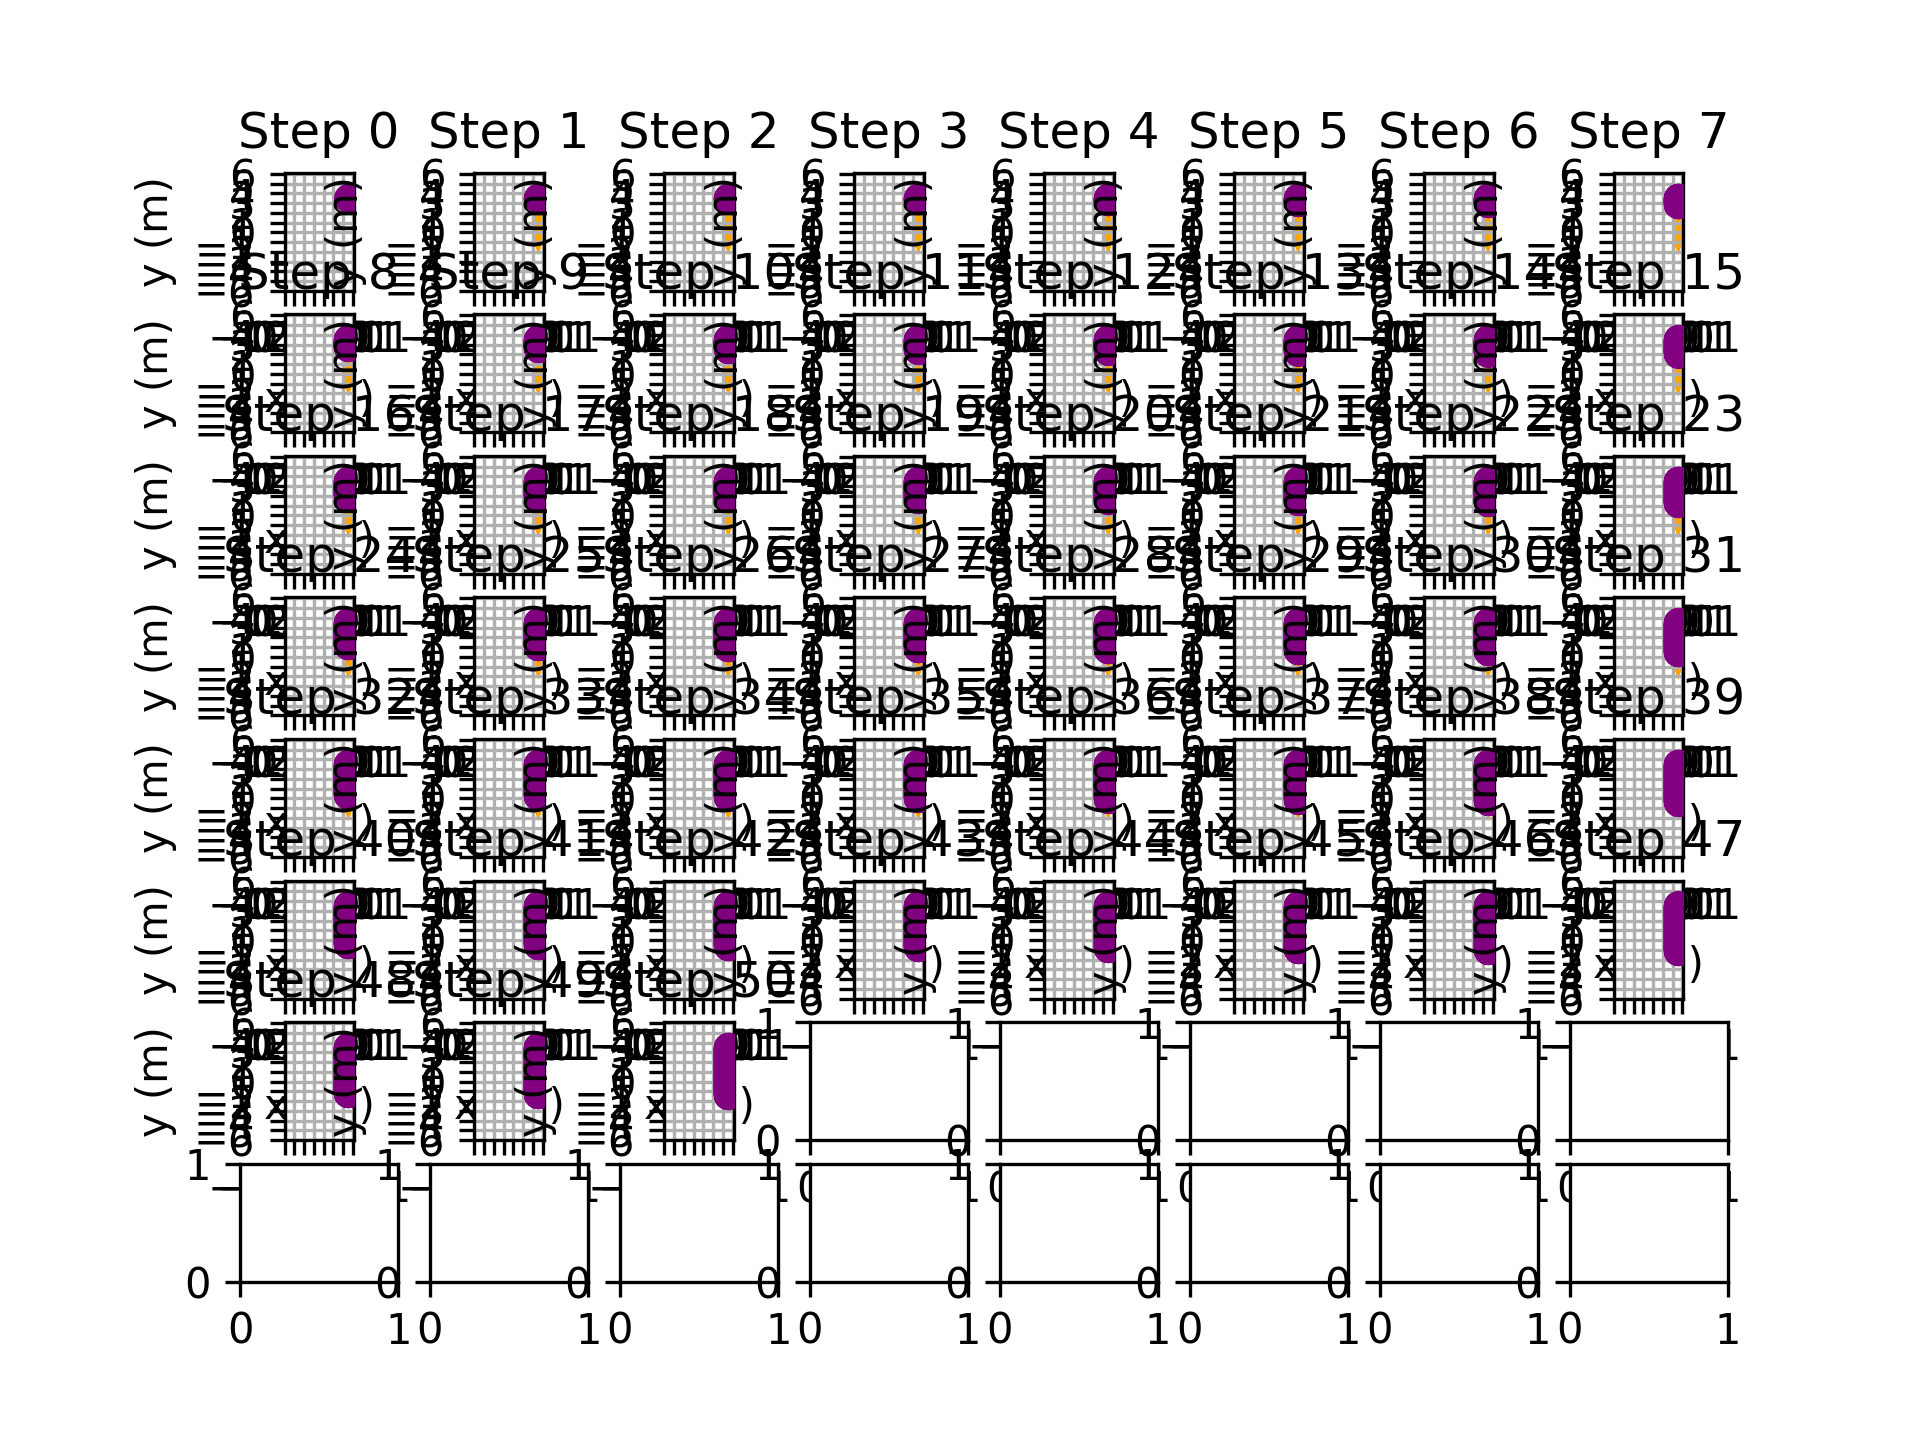
\includegraphics[width=0.4\textwidth]{"outputs/q11: #5.png"}
    \caption{Q11 Online Plan 3.B, cell-width 0.1.}
\end{figure}


\begin{figure}[H]
    \centering
    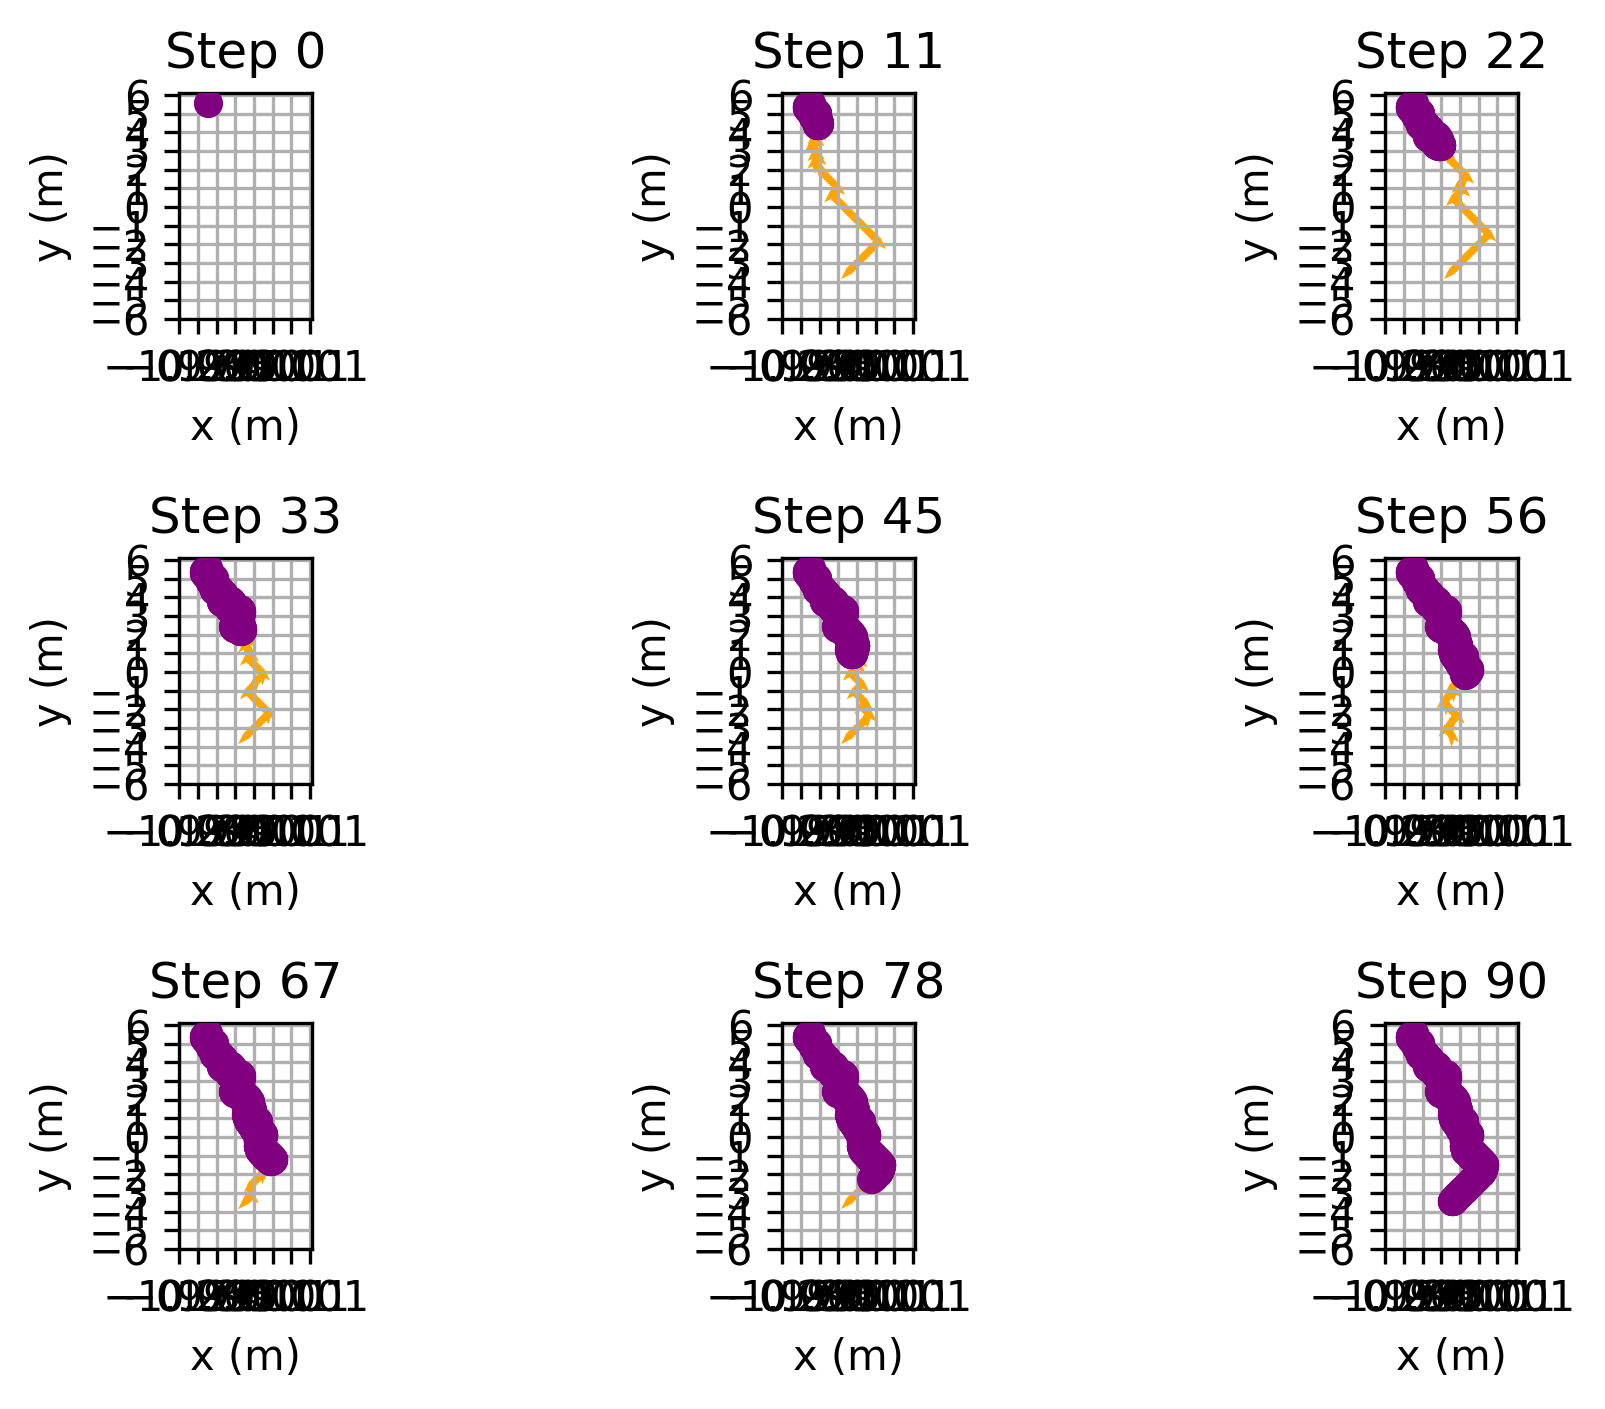
\includegraphics[width=0.5\textwidth]{"outputs/q11: #6.png"}
    \caption{Q11 Online Plan 3.C, cell-width 0.1.}
\end{figure}

\section{Question 12}
In the real world robot sensors may not give accurate readings for obstacle locations. Real robots also may not have a great estimation of their own state. For both of these issues, sensor fusion methods and SLAM methods may be integrated.

Maps limits may not be known beforehand.

Obstacles may be dynamic, thereby requiring more frequent re-plans.

Robots doing anything interesting may also need to receive goals from some mechanism, be it another classical algorithm, a human, or a machine learning agent. This may limit the amount of compute available to the path planner.

Real robots may have many more dimensions (ex: multi-fingered robot hands) for which grid-based search algorithms like A* don't scale.


\end{document}












